\chapter{Results}

This chapter presents detailed findings while preserving all figures and tables. We expand on mixture effects, learning-rate sensitivity, dataset size and format, and cross-dataset transfer patterns.

\begin{table}[h]
\centering
\caption{Overview of 10 pretraining experiments. Per dataset, we pretrain at 0.6B/1.7B/4B and evaluate on 8 test sets. LR adjustments are applied where noted.}
\label{tab:experiments_overview}
\resizebox{\textwidth}{!}{
\begin{tabular}{l l l l}
\toprule
\textbf{Experiment} & \textbf{Training source} & \textbf{Tokens} & \textbf{Notes} \\
\midrule
Mixed Financial & 7 financial datasets & 207M & 50\% capping (50cap) \;\; strong financial performance \\
Mixed Wiki+Financial & WikiText + 7 financial & $\sim$400M & Improves WikiText; degrades financial vs Mixed Financial \\
WikiText & WikiText-103 & 100M & General-domain baseline; LR sensitive at scale \\
Financial News & News articles & 197M & Long-form; low CV; good standalone \\
SEC Reports & Regulatory filings & 80M & Long-form; low CV; good standalone \\
FinGPT & Instruction mixture & 19M & Instruction format cluster \\
Alpaca (Finance) & Instruction mixture & 17M & Instruction format cluster \\
FiQA & Short Q\&A & 4M & Short-form; moderate CV \\
Financial QA 10K & Q\&A (10K examples) & 3.5M & Very small; high CV; LR tuning needed \\
Twitter Financial & Tweets & 0.3M & Very small; short-form outlier; highest CV \\
\bottomrule
\end{tabular}}
\end{table}

\section{Mixture Effects}
\textbf{Summary.} Mixed financial datasets outperform pure WikiText on all financial evaluations, and outperform Mixed Wiki+Financial when the objective is finance. Adding WikiText marginally improves general-domain performance but dilutes financial specialization.

\textbf{Evidence.} \Cref{fig:scaling_mixed_financial,fig:scaling_mixed_wiki_financial} visualize scaling across sizes; 4B Mixed Financial achieves 21.55 ppl (mean across financial sets), whereas Mixed Wiki+Financial degrades to 26.69 ppl despite gains on WikiText.

\begin{figure}[H]
  \centering
  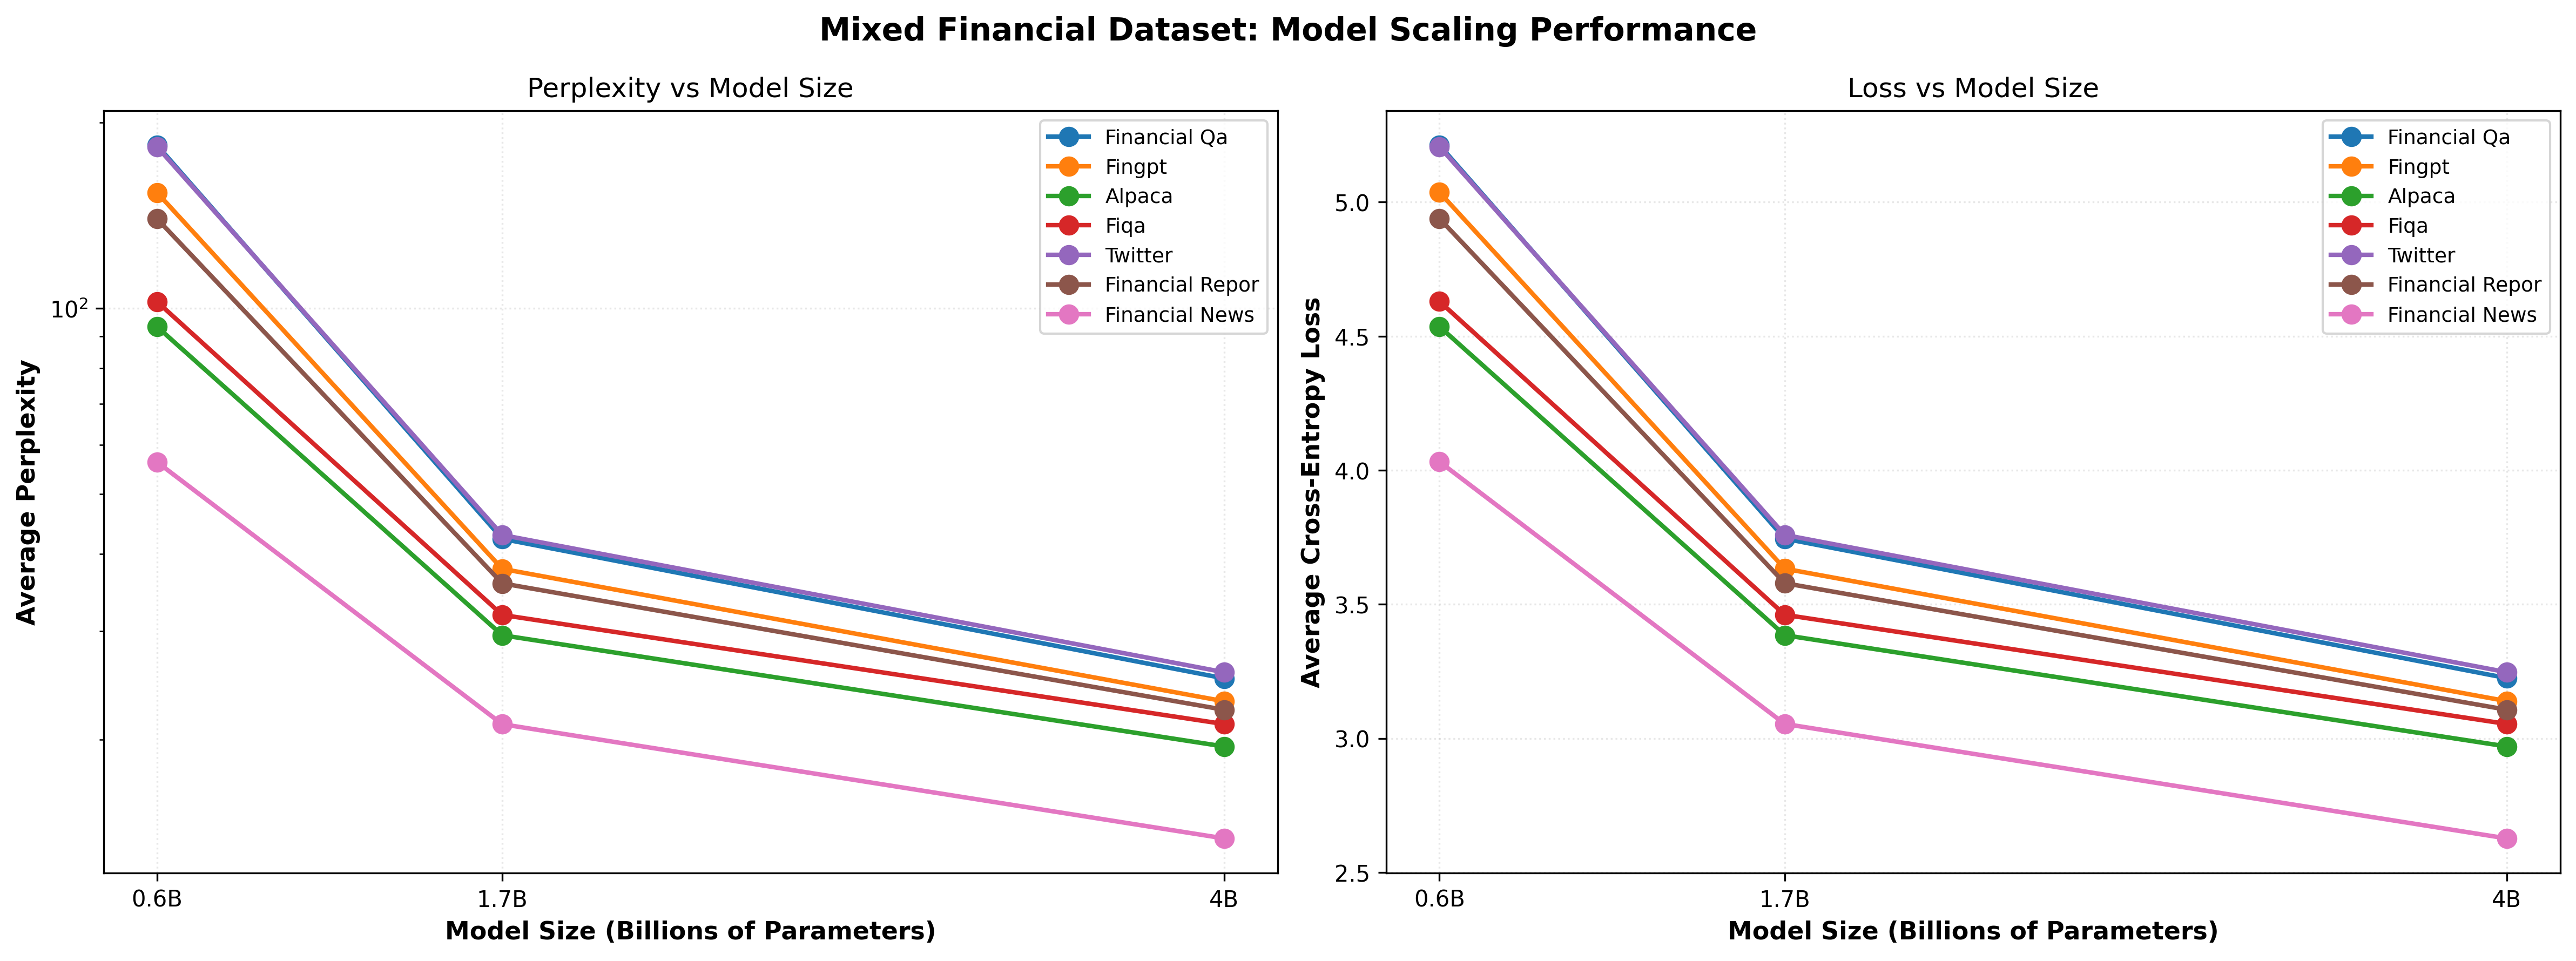
\includegraphics[width=\textwidth]{../thesis/figures/scaling_mixed_financial.png}
  \caption{Mixed Financial scaling.}\label{fig:scaling_mixed_financial}
\end{figure}

\begin{figure}[H]
  \centering
  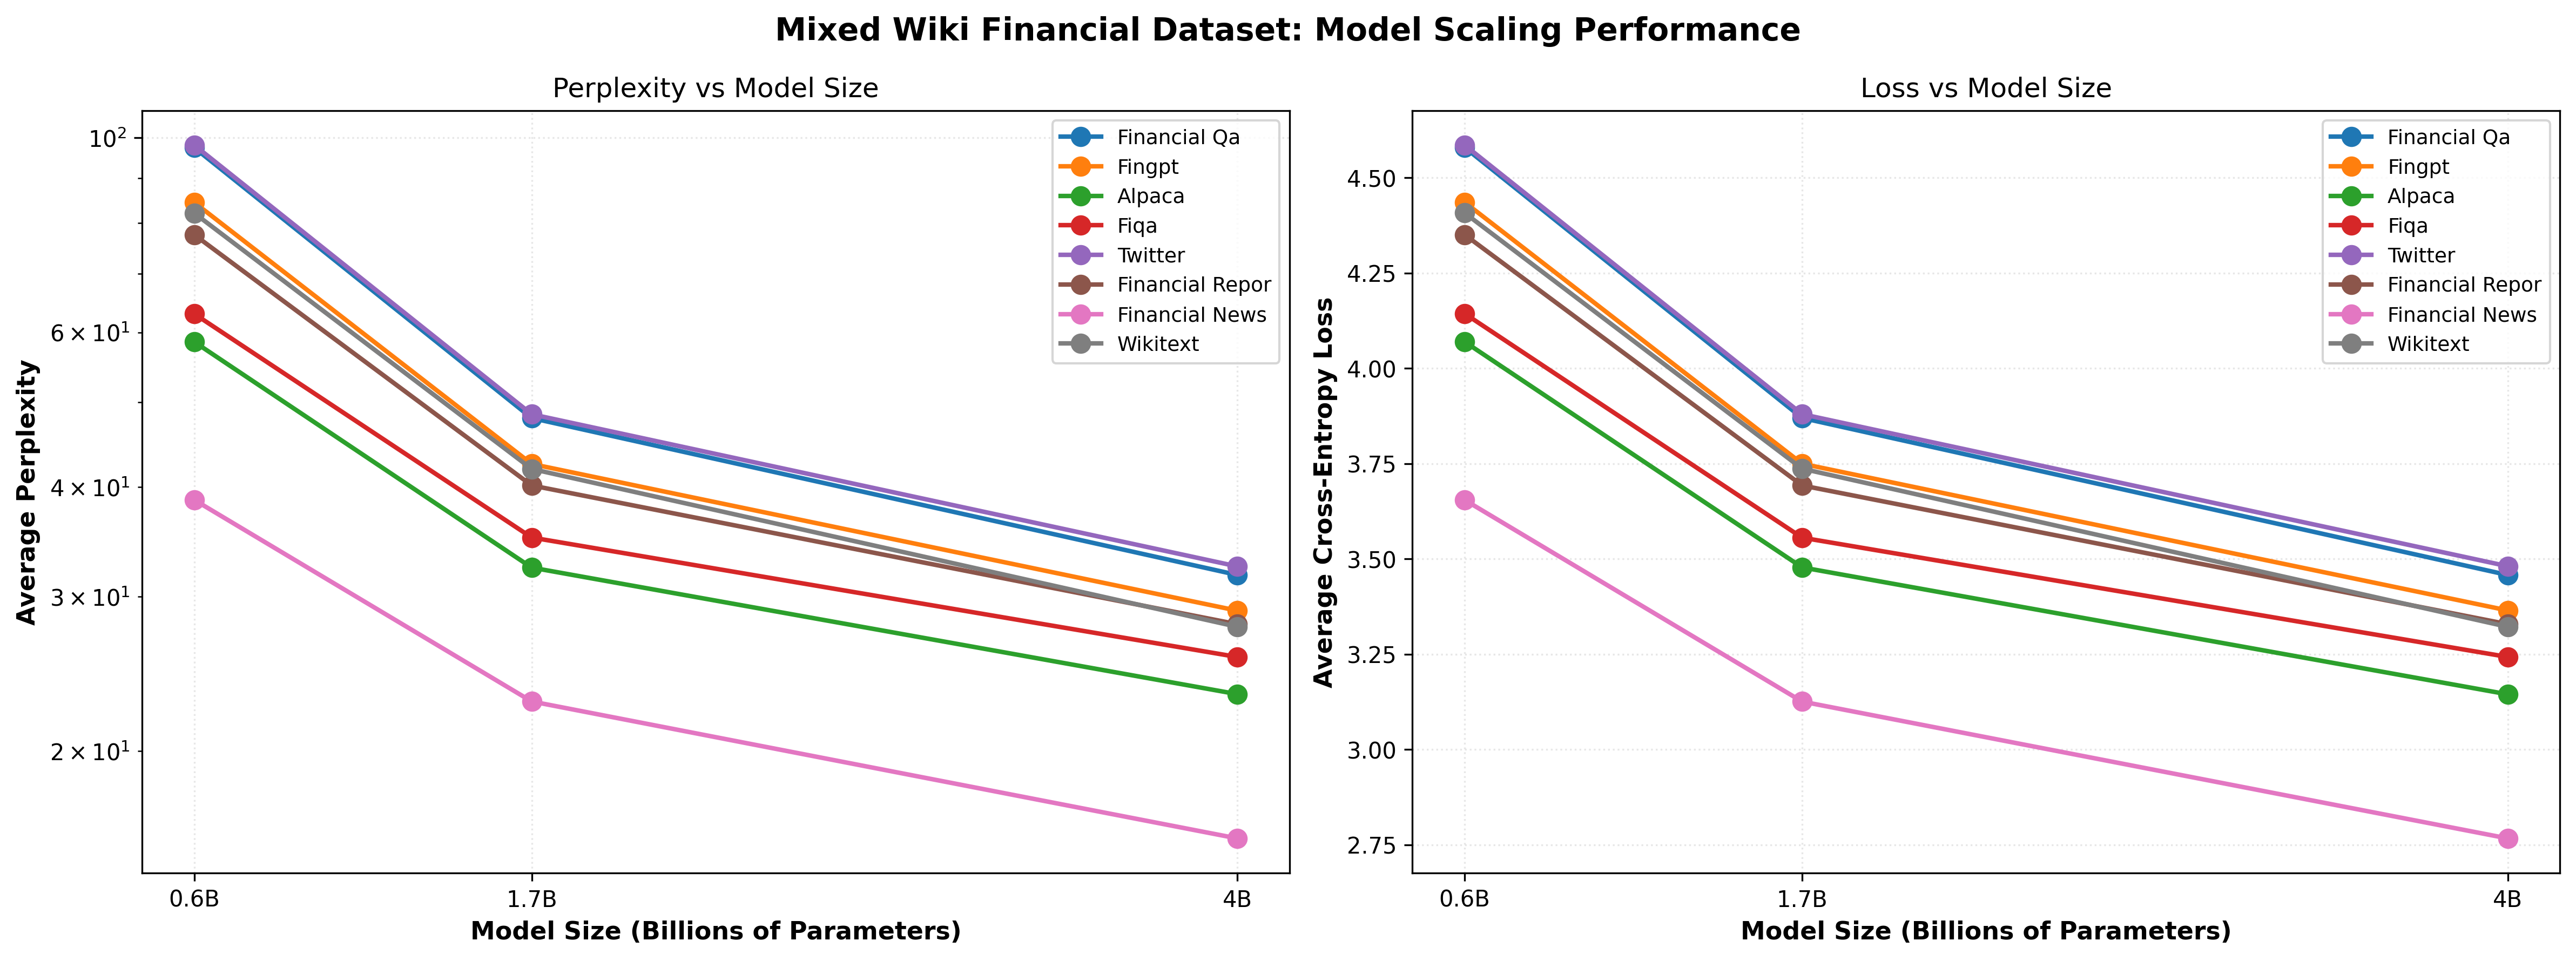
\includegraphics[width=\textwidth]{../thesis/figures/scaling_mixed_wiki_financial.png}
  \caption{Mixed Wiki+Financial scaling.}\label{fig:scaling_mixed_wiki_financial}
\end{figure}

{\tighttable
% Mixed Financial Dataset: Evaluation Results
% Training: Mixed Financial (7 datasets mixed, 322M tokens)
% All models trained with LR=2e-5

\begin{table}[h]
\centering
\caption{Mixed Financial Dataset: Evaluation Across Multiple Datasets}
\label{tab:mixed_financial_results}
\begin{tabular}{l|ccc|ccc}
\hline
\textbf{Eval Dataset} & \multicolumn{3}{c|}{\textbf{Cross-Entropy Loss}} & \multicolumn{3}{c}{\textbf{Perplexity}} \\
\cline{2-4} \cline{5-7}
  & \textbf{0.6B} & \textbf{1.7B} & \textbf{4B} & \textbf{0.6B} & \textbf{1.7B} & \textbf{4B} \\
\hline
Alpaca & 4.54 & 3.38 & \textbf{2.97} & 93.35 & \textbf{29.53} & \textbf{19.50} \\
Financial News & 4.03 & 3.05 & \textbf{2.63} & 56.35 & \textbf{21.19} & \textbf{13.84} \\
Financial Qa & 5.21 & 3.75 & \textbf{3.23} & 183.7 & \textbf{42.30} & \textbf{25.14} \\
Financial Repor & 4.94 & 3.58 & \textbf{3.11} & 139.6 & \textbf{35.83} & \textbf{22.36} \\
Fingpt & 5.04 & 3.63 & \textbf{3.14} & 153.9 & \textbf{37.82} & \textbf{23.08} \\
Fiqa & 4.63 & 3.46 & \textbf{3.05} & 102.5 & \textbf{31.85} & \textbf{21.20} \\
Twitter & 5.21 & 3.76 & \textbf{3.25} & 182.6 & \textbf{42.91} & \textbf{25.72} \\
\hline
\end{tabular}
\end{table}

}

The Mixed Financial table reports per-evaluation dataset loss and perplexity at 0.6B/1.7B/4B. The dominant pattern is that 4B consistently wins (bolded minima), with the largest gap on long-form document sets (News, SEC), and smaller but persistent gains on instruction/short-form (FinGPT, Alpaca, FiQA). This confirms that in-domain diversity plus model capacity improves both specialization and robustness.

{\tighttable
% Mixed Wiki+Financial Dataset: Evaluation Results
% Training: Mixed Wiki+Financial (WikiText + 7 financial datasets, ~400M tokens)
% All models trained with LR=2e-5

\begin{table}[h]
\centering
\caption{Mixed Wiki+Financial Dataset: Evaluation Across Multiple Datasets}
\label{tab:mixed_wiki_financial_results}
\resizebox{\textwidth}{!}{
\begin{tabular}{l|ccc|ccc}
\toprule
\multirow{2}{*}{\textbf{Eval Dataset}} &
\multicolumn{3}{c|}{\textbf{Cross-Entropy Loss}} &
\multicolumn{3}{c}{\textbf{Perplexity}} \\
\cmidrule(lr){2-4} \cmidrule(lr){5-7}
& \textbf{0.6B} & \textbf{1.7B} & \textbf{4B} & \textbf{0.6B} & \textbf{1.7B} & \textbf{4B} \\
\midrule
Alpaca & 4.07 & 3.48 & 3.15 & 58.56 & 32.38 & 23.23 \\
Financial News & 3.65 & 3.13 & 2.77 & 38.68 & 22.79 & 15.91 \\
Financial Qa & 4.58 & 3.87 & 3.46 & 97.49 & 47.94 & 31.76 \\
Financial Repor & 4.35 & 3.69 & 3.33 & 77.57 & 40.17 & 27.91 \\
Fingpt & 4.44 & 3.75 & 3.37 & 84.43 & 42.50 & 28.92 \\
Fiqa & 4.14 & 3.56 & 3.24 & 63.03 & 35.04 & 25.61 \\
Twitter & 4.59 & 3.88 & 3.48 & 98.13 & 48.42 & 32.48 \\
Wikitext & 4.41 & 3.74 & 3.32 & 82.10 & 41.95 & 27.72 \\
\bottomrule
\end{tabular}
}
\end{table}

}

The Mixed Wiki+Financial table shows that mixing in general text helps on WikiText but hurts on all financial evaluations relative to Mixed Financial (previous table). The degradation is largest on long-form sets, indicating that the added general-domain mass reduces effective exposure to financial discourse structure.

\section{Scaling and LR Sensitivity}
\textbf{Reverse scaling and fix.} With a constant LR, 1.7B/4B sometimes underperform 0.6B (``reverse scaling''). Adjusting LR by size resolves this. Empirically, reducing LR roughly with $1/\sqrt{N}$ restores expected ordering and improves 10--32\%.

\textbf{Evidence.} \Cref{fig:scaling_wikitext,fig:scaling_financial_qa,fig:scaling_twitter} compare original vs adjusted LRs (solid vs dashed). The next three tables report the corresponding per-dataset improvements and average recovery.

\begin{figure}[H]
  \centering
  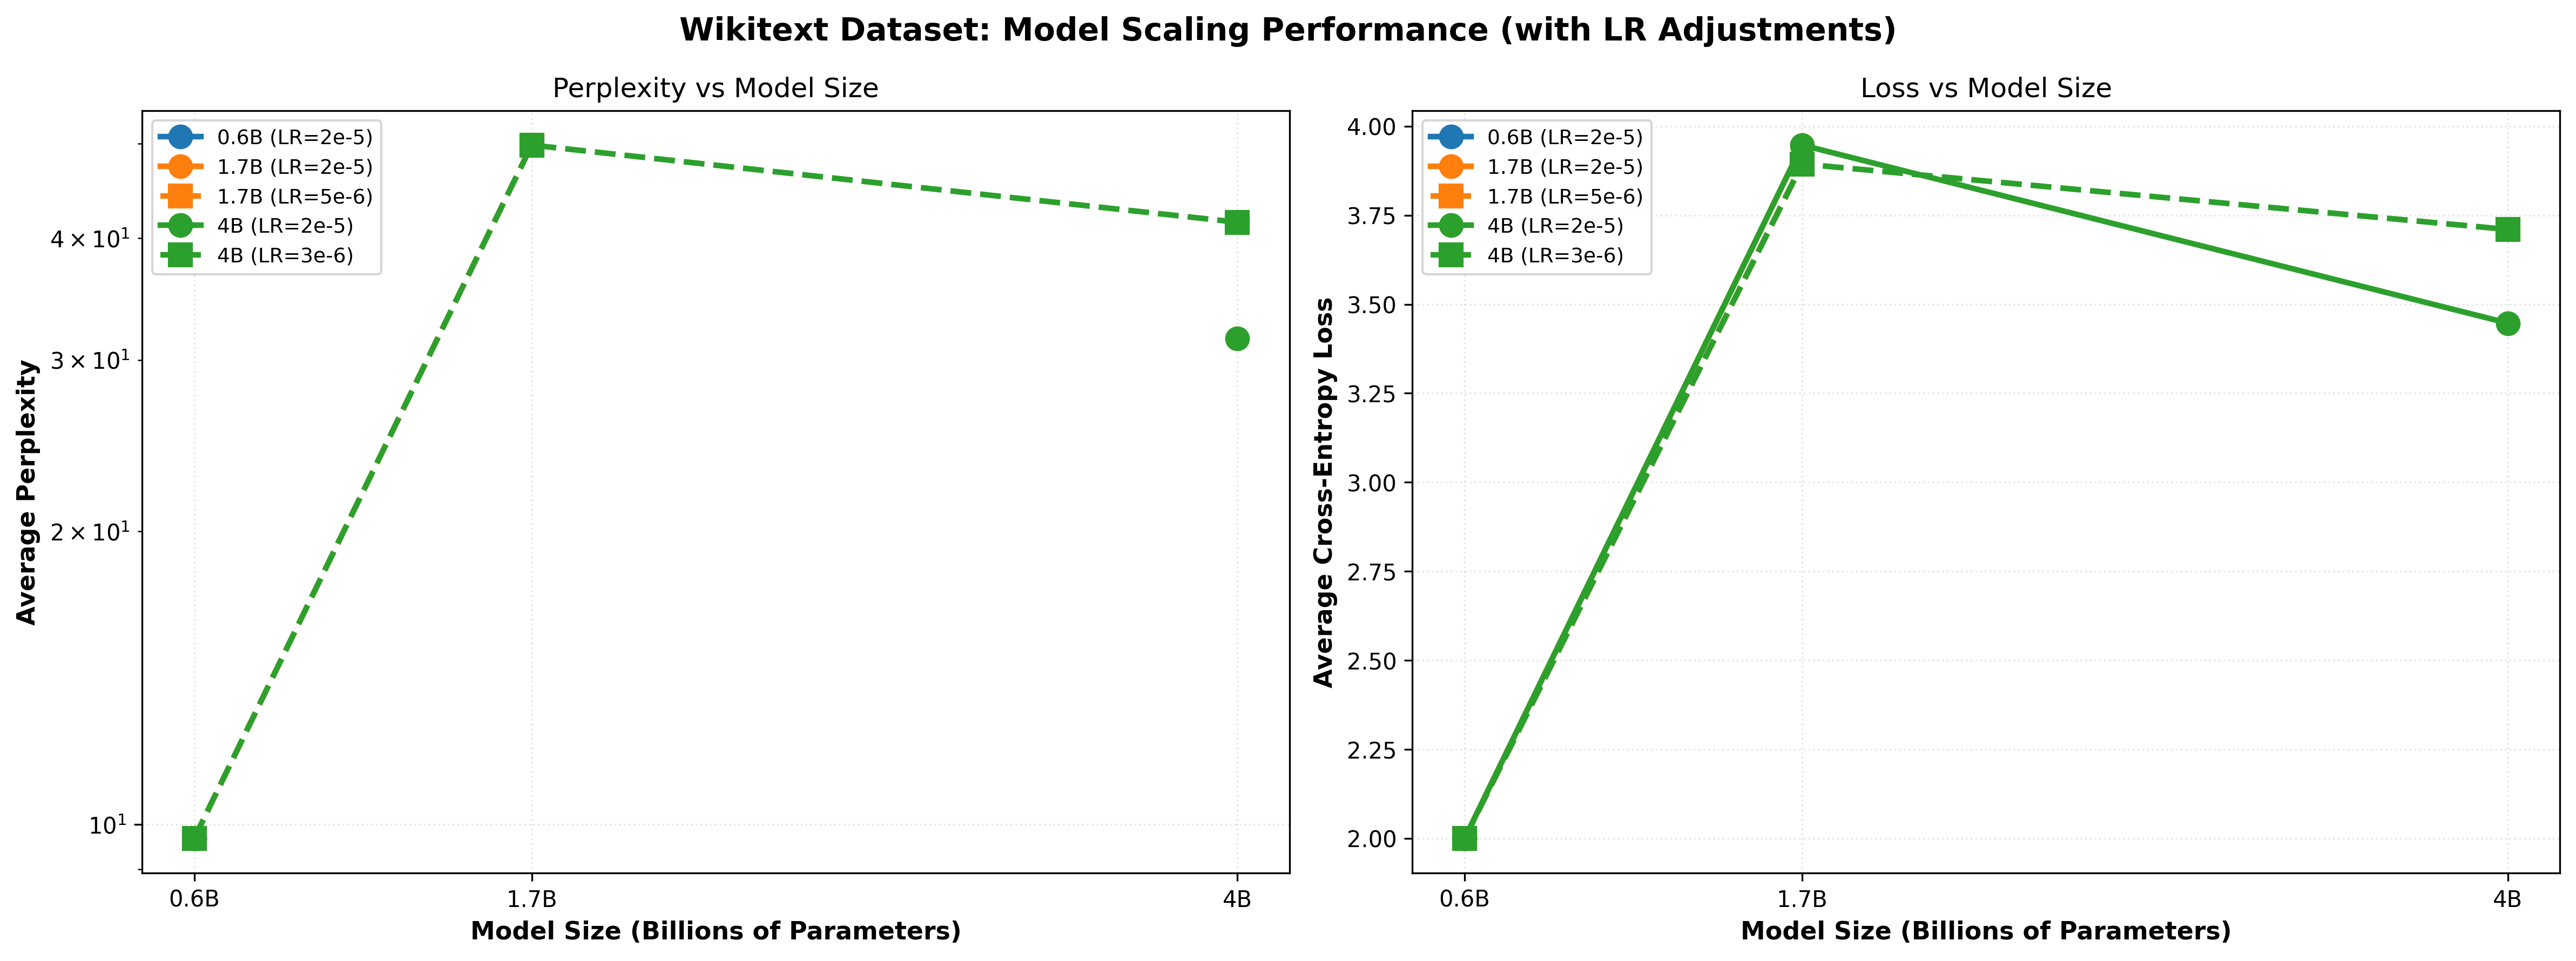
\includegraphics[width=\textwidth]{../thesis/figures/scaling_wikitext.png}
  \caption{WikiText LR comparison.}\label{fig:scaling_wikitext}
\end{figure}

{\tighttable
% WikiText Dataset: Evaluation Results with LR Adjustments
% Training: WikiText (WikiText-103, 100M tokens)
% LR Adjustments: 1.7B (2e-5 → 5e-6), 4B (2e-5 → 3e-6)

\begin{table}[h]
\centering
\caption[WikiText: Learning Rate Comparison]{WikiText Dataset: Impact of Learning Rate Adjustments}
\label{tab:wikitext_lr_comparison}
\begin{tabular}{l|c|cc|cc|c|cc|cc}
\hline
\multirow{3}{*}{\textbf{Eval Dataset}} &
\multicolumn{5}{c|}{\textbf{Cross-Entropy Loss}} &
\multicolumn{5}{c}{\textbf{Perplexity}} \\
\cline{2-6} \cline{7-11}
& \textbf{0.6B} & \multicolumn{2}{c|}{\textbf{1.7B}} & \multicolumn{2}{c|}{\textbf{4B}} &
 \textbf{0.6B} & \multicolumn{2}{c|}{\textbf{1.7B}} & \multicolumn{2}{c}{\textbf{4B}} \\
\cline{3-4} \cline{5-6} \cline{8-9} \cline{10-11}
& \textbf{2e-5} & \textbf{2e-5} & \textbf{5e-6} & \textbf{2e-5} & \textbf{3e-6} &
 \textbf{2e-5} & \textbf{2e-5} & \textbf{5e-6} & \textbf{2e-5} & \textbf{3e-6} \\
\hline
 Alpaca & 2.22 & \textbf{3.24} & 3.79 & \textbf{3.48} & 3.64 & 9.23 & \textbf{25.51} & 44.22 & \textbf{32.38} & 38.06 \\
Financial News & 2.62 & \textbf{2.93} & 3.52 & 3.37 & \textbf{3.27} & 13.70 & \textbf{18.78} & 33.66 & \textbf{29.19} & \textbf{26.44} \\
 Financial QA & 3.40 & 10.67 & \textbf{4.07} & \textbf{3.37} & 3.87 & 29.90 & $\infty$ & \textbf{58.33} & \textbf{29.08} & 47.98 \\
 SEC Reports & 1.39 & \textbf{3.27} & 3.91 & \textbf{3.44} & 3.75 & 3.99 & \textbf{26.46} & 49.83 & \textbf{31.23} & 42.41 \\
 FinGPT & 1.30 & \textbf{2.11} & 4.07 & \textbf{3.57} & 3.88 & 3.67 & \textbf{8.27} & 58.55 & \textbf{35.50} & 48.30 \\
 FiQA & 2.07 & \textbf{3.14} & 3.85 & \textbf{3.53} & 3.74 & 7.89 & \textbf{23.15} & 46.81 & \textbf{34.03} & 42.04 \\
Twitter & 1.45 & \textbf{2.78} & 4.08 & \textbf{3.52} & 3.88 & 4.26 & \textbf{16.06} & 58.98 & \textbf{33.71} & 48.48 \\
\rowcolor{gray!20} \textbf{Wikitext (train)} & 1.56 & \textbf{3.42} & 3.88 & \textbf{3.30} & 3.65 & 4.78 & \textbf{30.63} & 48.44 & \textbf{27.19} & 38.60 \\
\rowcolor{blue!10} \textbf{Average} & \textbf{2.00} & \textbf{3.95} & \textbf{3.89} & \textbf{3.45} & \textbf{3.71} & \textbf{9.68} & \textbf{$\infty$} & \textbf{49.85} & \textbf{31.54} & \textbf{41.54}  \\
\hline
\end{tabular}
\end{table}
}

\begin{figure}[H]
  \centering
  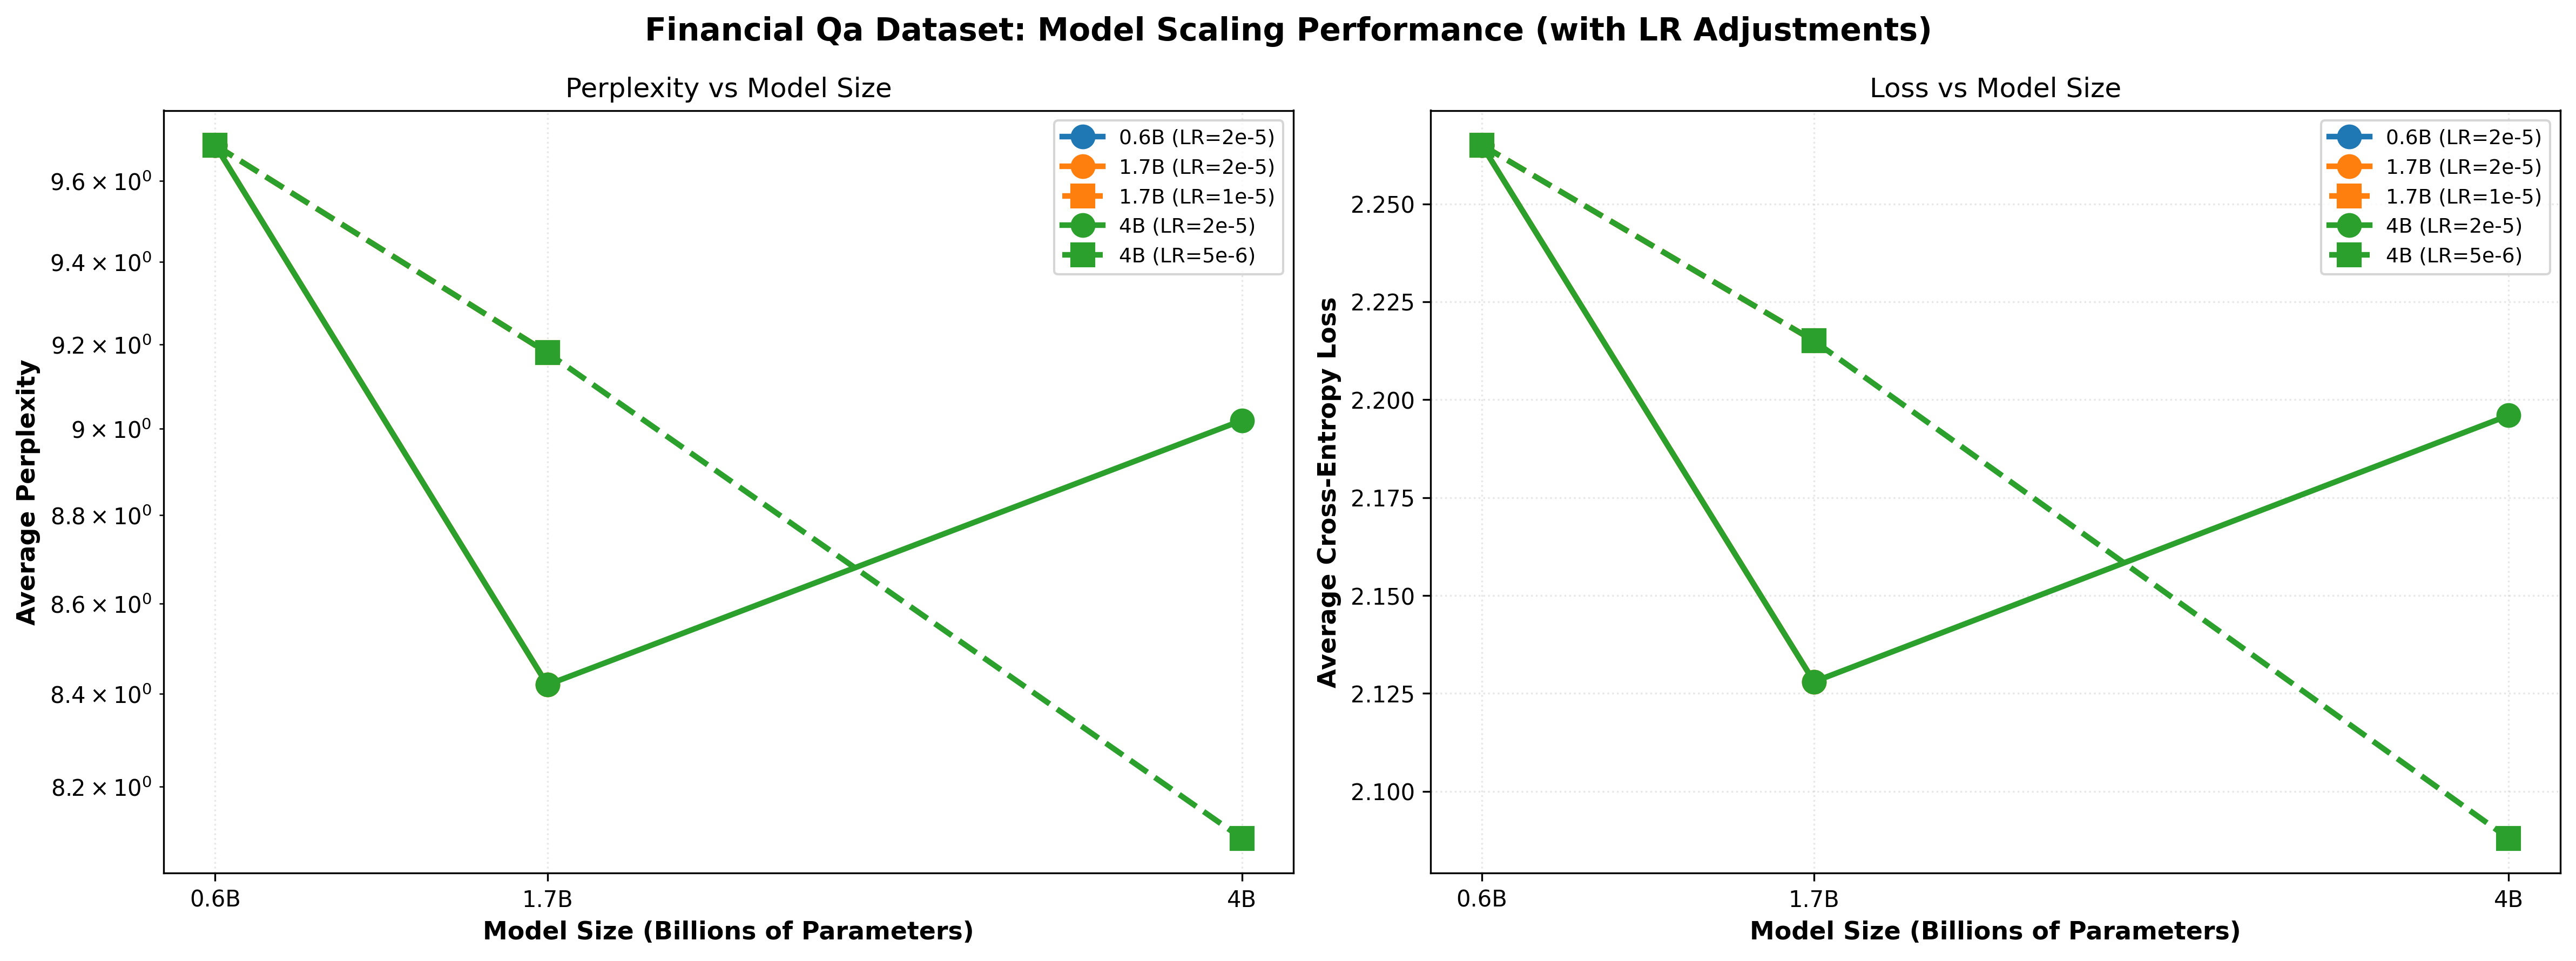
\includegraphics[width=\textwidth]{../thesis/figures/scaling_financial_qa.png}
  \caption{Financial QA: LR adjustment resolves reverse scaling.}\label{fig:scaling_financial_qa}
\end{figure}

{\tighttable
% Financial QA 10K Dataset: Evaluation Results with LR Adjustments
% Training: Financial QA 10K (virattt/financial-qa-10K, 3.5M tokens)
% LR Adjustments: 1.7B (2e-5 → 1e-5), 4B (2e-5 → 5e-6)

\begin{table}[h]
\centering
\caption[Financial QA 10K: Learning Rate Comparison]{Financial QA 10K Dataset: Impact of Learning Rate Adjustments}
\label{tab:financial_qa_lr_comparison}
\begin{tabular}{l|c|cc|cc|c|cc|cc}
\hline
\multirow{3}{*}{\textbf{Eval Dataset}} &
\multicolumn{5}{c|}{\textbf{Cross-Entropy Loss}} &
\multicolumn{5}{c}{\textbf{Perplexity}} \\
\cline{2-6} \cline{7-11}
& \textbf{0.6B} & \multicolumn{2}{c|}{\textbf{1.7B}} & \multicolumn{2}{c|}{\textbf{4B}} &
 \textbf{0.6B} & \multicolumn{2}{c|}{\textbf{1.7B}} & \multicolumn{2}{c}{\textbf{4B}} \\
\cline{3-4} \cline{5-6} \cline{8-9} \cline{10-11}
& \textbf{2e-5} & \textbf{2e-5} & \textbf{1e-5} & \textbf{2e-5} & \textbf{5e-6} &
 \textbf{2e-5} & \textbf{2e-5} & \textbf{1e-5} & \textbf{2e-5} & \textbf{5e-6} \\
\hline
 Alpaca & 2.38 & \textbf{2.23} & 2.29 & 2.29 & \textbf{2.18} & 10.82 & \textbf{9.31} & 9.92 & \textbf{9.91} & \textbf{8.88} \\
Financial News & 2.36 & \textbf{2.17} & 2.23 & 2.13 & \textbf{2.04} & 10.60 & \textbf{8.78} & 9.25 & \textbf{8.41} & \textbf{7.71} \\
\rowcolor{gray!20} \textbf{Financial QA (train)} & 2.12 & \textbf{2.01} & 2.12 & 2.12 & \textbf{2.01} & 8.29 & \textbf{7.44} & 8.29 & 8.29 & \textbf{7.43} \\
SEC Reports & 2.11 & \textbf{2.00} & 2.10 & 2.11 & \textbf{2.01} & 8.21 & \textbf{7.40} & 8.19 & \textbf{8.25} & \textbf{7.43} \\
FinGPT & 2.31 & \textbf{2.15} & 2.25 & 2.23 & \textbf{2.11} & 10.04 & \textbf{8.62} & 9.51 & \textbf{9.34} & \textbf{8.24} \\
FiQA & 2.40 & \textbf{2.25} & 2.31 & 2.31 & \textbf{2.19} & 11.02 & \textbf{9.45} & 10.10 & \textbf{10.05} & \textbf{8.93} \\
Twitter & 2.21 & \textbf{2.10} & 2.21 & 2.20 & \textbf{2.09} & 9.14 & \textbf{8.18} & 9.10 & \textbf{8.99} & \textbf{8.05} \\
Wikitext & 2.24 & \textbf{2.11} & 2.21 & 2.19 & \textbf{2.08} & 9.41 & \textbf{8.23} & 9.08 & \textbf{8.89} & \textbf{8.00} \\
\rowcolor{blue!10} \textbf{Average} & \textbf{2.27} & \textbf{2.13} & \textbf{2.21} & \textbf{2.20} & \textbf{2.09} & \textbf{9.69} & \textbf{8.42} & \textbf{9.18} & \textbf{9.02} & \textbf{8.09}  \\
\hline
\end{tabular}
\end{table}
}

\begin{figure}[H]
  \centering
  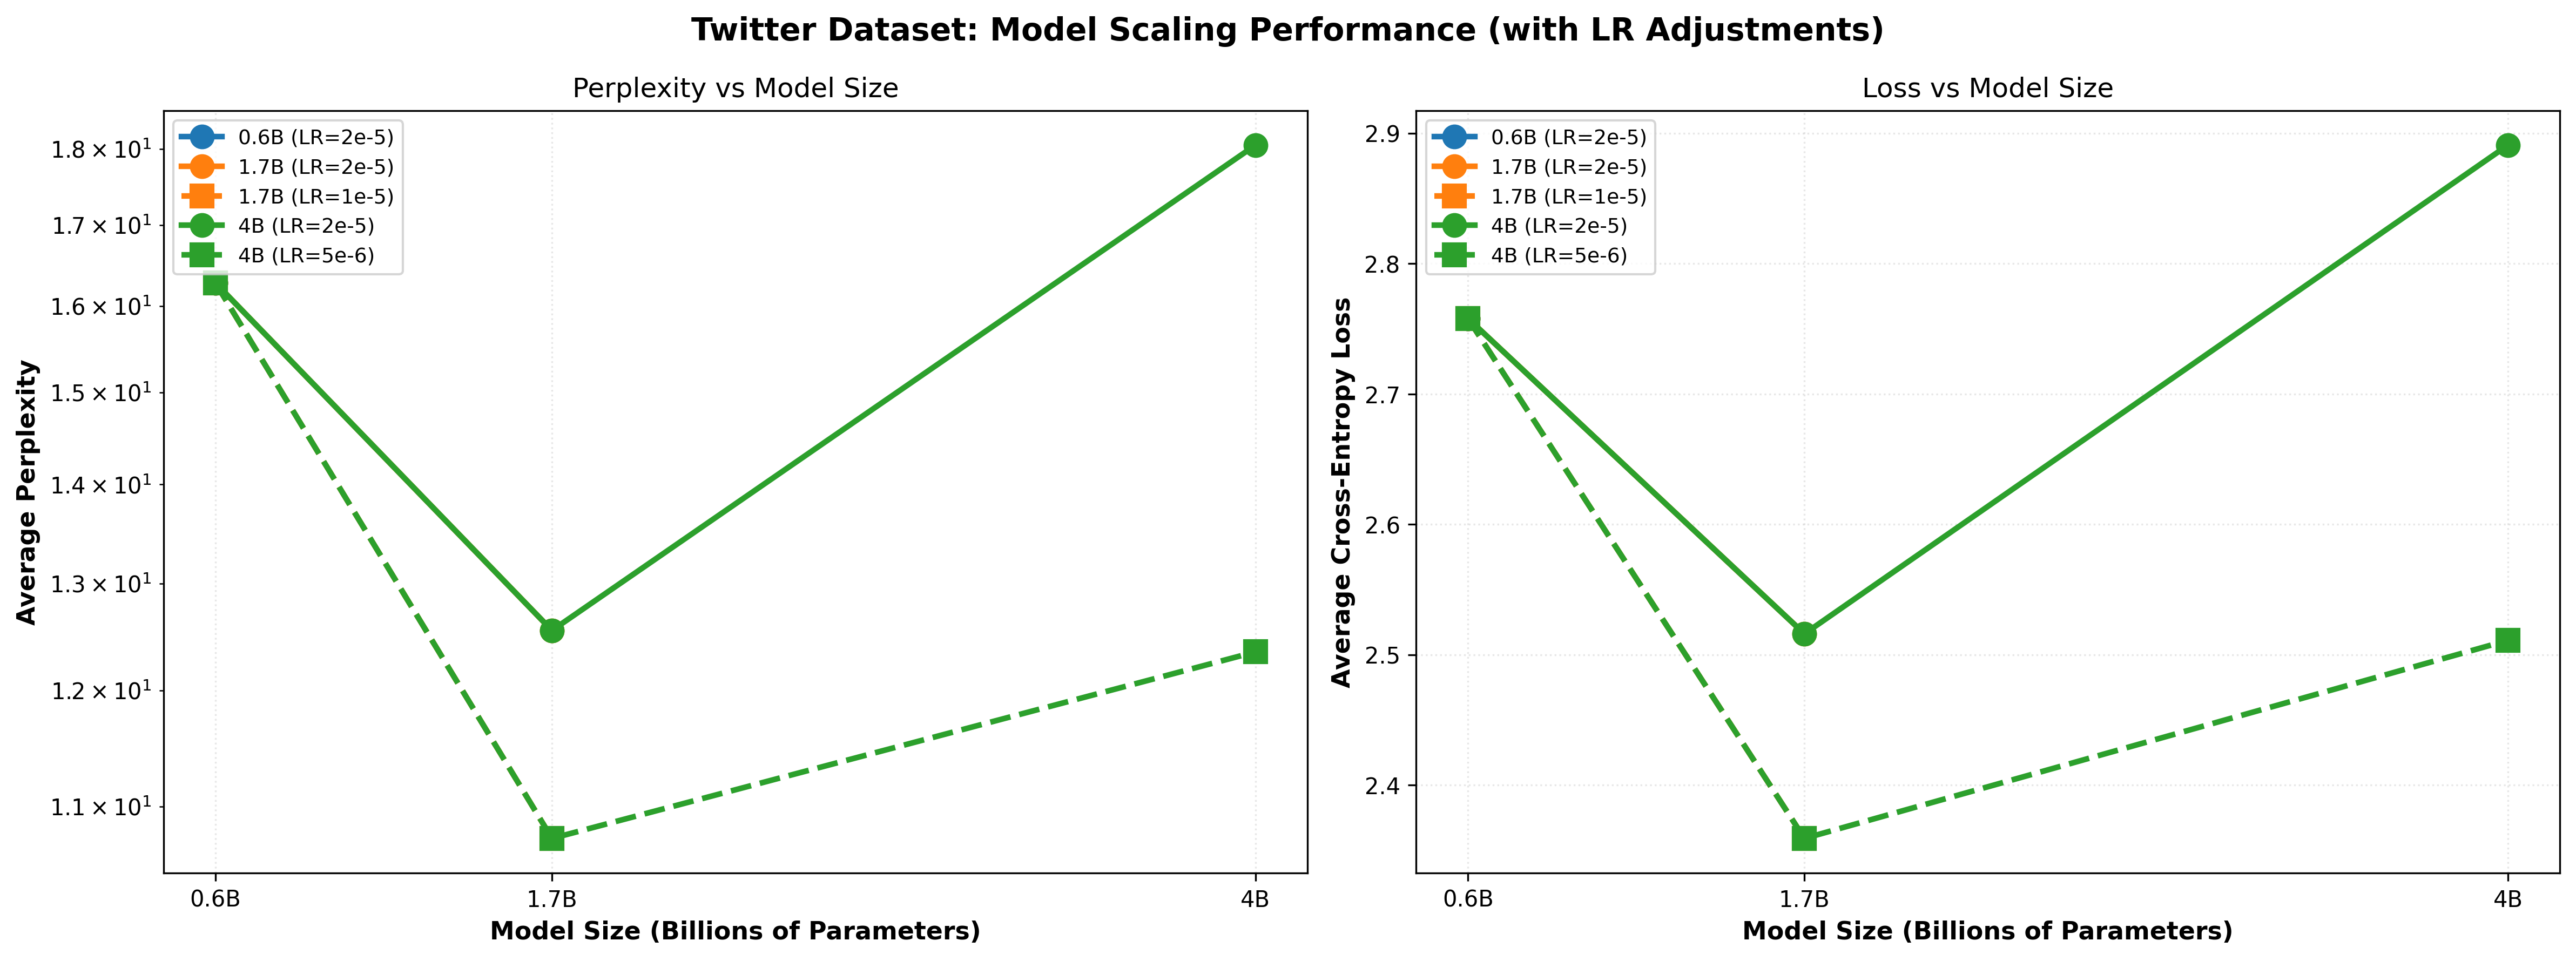
\includegraphics[width=\textwidth]{../thesis/figures/scaling_twitter.png}
  \caption{Twitter: severe LR sensitivity at small data scales.}\label{fig:scaling_twitter}
\end{figure}

{\tighttable
% Twitter Financial Dataset: Evaluation Results with LR Adjustments
% Training: Twitter Financial (Financial tweets, 0.28M tokens)
% LR Adjustments: 1.7B (2e-5 → 1e-5), 4B (2e-5 → 5e-6)

\begin{table}[h]
\centering
\caption[Twitter Financial: Learning Rate Comparison]{Twitter Financial Dataset: Impact of Learning Rate Adjustments}
\label{tab:twitter_lr_comparison}
\begin{tabular}{l|c|cc|cc|c|cc|cc}
\hline
\multirow{3}{*}{\textbf{Eval Dataset}} &
\multicolumn{5}{c|}{\textbf{Cross-Entropy Loss}} &
\multicolumn{5}{c}{\textbf{Perplexity}} \\
\cline{2-6} \cline{7-11}
& \textbf{0.6B} & \multicolumn{2}{c|}{\textbf{1.7B}} & \multicolumn{2}{c|}{\textbf{4B}} &
 \textbf{0.6B} & \multicolumn{2}{c|}{\textbf{1.7B}} & \multicolumn{2}{c}{\textbf{4B}} \\
\cline{3-4} \cline{5-6} \cline{8-9} \cline{10-11}
& \textbf{2e-5} & \textbf{2e-5} & \textbf{1e-5} & \textbf{2e-5} & \textbf{5e-6} &
 \textbf{2e-5} & \textbf{2e-5} & \textbf{1e-5} & \textbf{2e-5} & \textbf{5e-6} \\
\hline
 Alpaca & 3.01 & 2.66 & \textbf{2.54} & 2.96 & \textbf{2.61} & 20.21 & 14.33 & \textbf{12.66} & \textbf{19.20} & \textbf{13.65} \\
Financial News & 3.17 & 2.80 & \textbf{2.65} & 2.87 & \textbf{2.54} & 23.77 & 16.48 & \textbf{14.10} & \textbf{17.67} & \textbf{12.68} \\
Financial QA & 2.46 & 2.32 & \textbf{2.16} & 2.83 & \textbf{2.43} & 11.76 & 10.15 & \textbf{8.69} & \textbf{16.98} & \textbf{11.39} \\
SEC Reports & 2.48 & 2.32 & \textbf{2.16} & 2.80 & \textbf{2.39} & 11.95 & 10.17 & \textbf{8.70} & \textbf{16.42} & \textbf{10.93} \\
FinGPT & 2.74 & 2.50 & \textbf{2.34} & 2.91 & \textbf{2.54} & 15.53 & 12.23 & \textbf{10.41} & \textbf{18.34} & \textbf{12.69} \\
FiQA & 2.98 & 2.66 & \textbf{2.50} & 3.00 & \textbf{2.61} & 19.67 & 14.26 & \textbf{12.20} & \textbf{20.09} & \textbf{13.61} \\
\rowcolor{gray!20} \textbf{Twitter (train)} & 2.53 & 2.40 & \textbf{2.22} & 2.88 & \textbf{2.47} & 12.60 & 11.02 & \textbf{9.21} & 17.83 & \textbf{11.81} \\
Wikitext & 2.69 & 2.47 & \textbf{2.30} & 2.88 & \textbf{2.49} & 14.74 & 11.78 & \textbf{9.94} & \textbf{17.85} & \textbf{12.02} \\
\rowcolor{blue!10} \textbf{Average} & \textbf{2.76} & \textbf{2.52} & \textbf{2.36} & \textbf{2.89} & \textbf{2.51} & \textbf{16.28} & \textbf{12.55} & \textbf{10.74} & \textbf{18.05} & \textbf{12.35}  \\
\hline
\end{tabular}
\end{table}
}

Across all three LR studies, the tuned LR eliminates training collapse (e.g., $\infty$ perplexity at 1.7B on WikiText), and recovers the expected monotone trend with model size. The average row in each table highlights meaningful gains at 1.7B and 4B while keeping 0.6B intact.

\section{Dataset Size and Format}
\textbf{Size thresholds.} Large datasets (News: 197M tokens; SEC: 80M) sustain standalone pretraining with low variance (26--32\% CV). Small datasets (Financial QA: 3.5M; Twitter: 0.3M) severely overtrain (tens to hundreds of epochs) and exhibit high variance (up to 89\% CV), motivating mixtures.

\textbf{Format matters.} Transfer depends strongly on format: long-form document models (News, SEC) transfer across each other better than to short-form (Twitter) or instruction formats (FinGPT/Alpaca); instruction-tuned sources cluster; short-form Twitter remains an outlier. Figures \Cref{fig:scaling_news_articles,fig:scaling_sec_reports,fig:scaling_fingpt,fig:scaling_alpaca,fig:scaling_fiqa} illustrate scaling within format families. The following single-source result tables quantify these trends.

\begin{figure}[H]
  \centering
  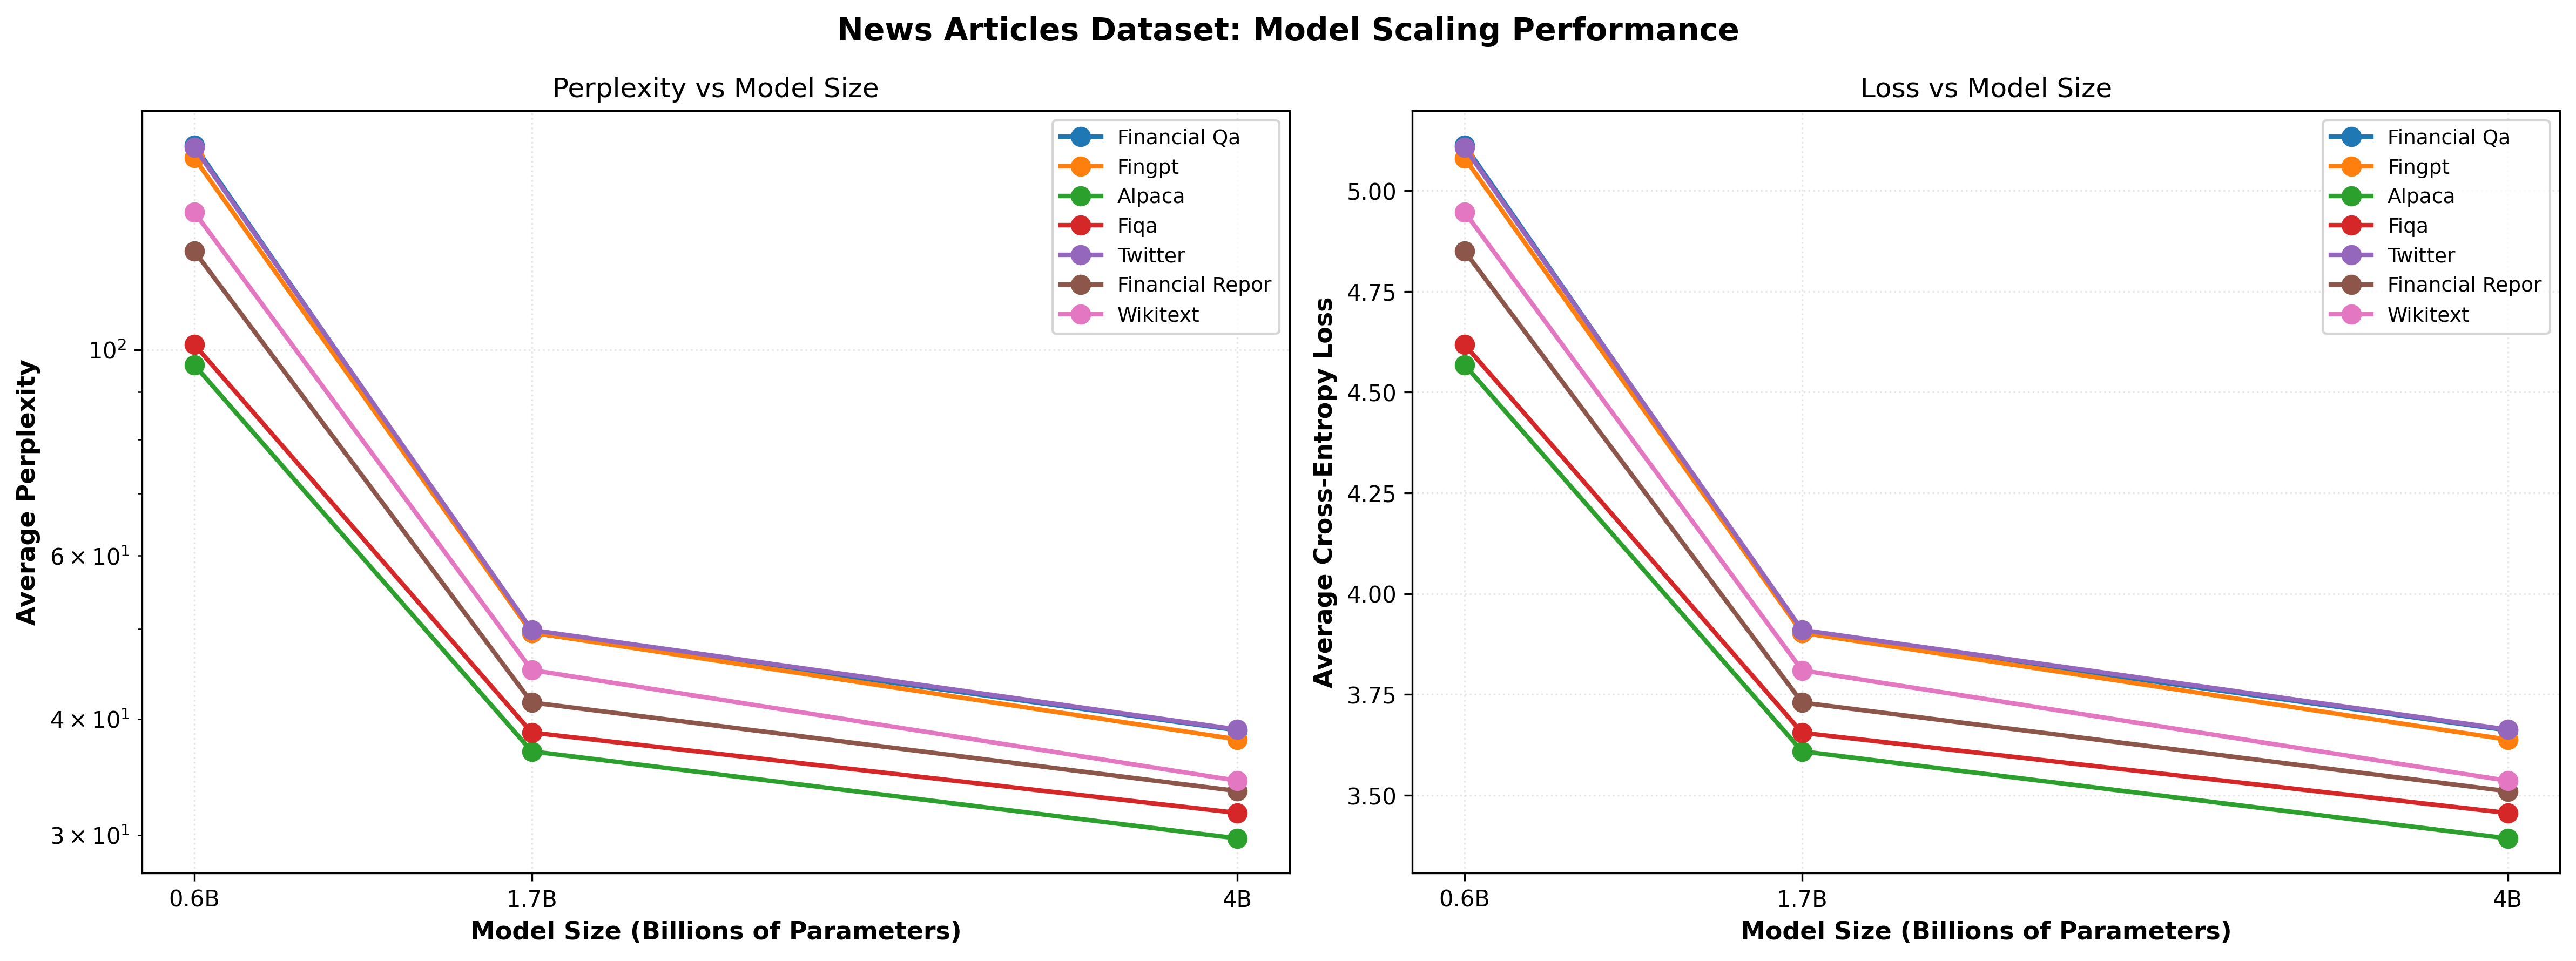
\includegraphics[width=\textwidth]{../thesis/figures/scaling_news_articles.png}
  \caption{News Articles scaling.}\label{fig:scaling_news_articles}
\end{figure}

{\tighttable
% Financial News Dataset: Evaluation Results
% Training: Financial News (Financial news articles, 194.47M tokens)
% All models trained with LR=2e-5

\begin{table}[htbp]
\centering
\caption[Financial News: Evaluation Results]{Financial News Dataset: Evaluation Across Multiple Datasets}
\label{tab:news_articles_results}
\begin{tabular}{l|ccc|ccc}
\hline
\textbf{Eval Dataset} & \multicolumn{3}{c|}{\textbf{Cross-Entropy Loss}} & \multicolumn{3}{c}{\textbf{Perplexity}} \\
\cline{2-4} \cline{5-7}
  & \textbf{0.6B} & \textbf{1.7B} & \textbf{4B} & \textbf{0.6B} & \textbf{1.7B} & \textbf{4B} \\
\hline
Alpaca & 4.57 & 3.61 & \textbf{3.39} & 96.31 & \textbf{36.92} & \textbf{29.75} \\
\textbf{Financial News} & \textbf{3.96} & \textbf{3.13} & \textbf{2.86} & \textbf{52.25} & \textbf{22.91} & \textbf{17.47} \\
Financial QA & 5.11 & 3.90 & \textbf{3.66} & 166.1 & \textbf{49.53} & \textbf{38.90} \\
SEC Reports & 4.85 & 3.73 & \textbf{3.51} & 127.7 & \textbf{41.68} & \textbf{33.46} \\
FinGPT & 5.08 & 3.90 & \textbf{3.64} & 160.9 & \textbf{49.56} & \textbf{38.03} \\
FiQA & 4.62 & 3.65 & \textbf{3.46} & 101.3 & \textbf{38.68} & \textbf{31.69} \\
Twitter & 5.11 & 3.91 & \textbf{3.66} & 165.2 & \textbf{49.88} & \textbf{38.98} \\
Wikitext & 4.95 & 3.81 & \textbf{3.54} & 140.7 & \textbf{45.17} & \textbf{34.33} \\
\hline
\textbf{Average} & \textbf{4.78} & \textbf{3.71} & \textbf{3.47} & \textbf{126.3} & \textbf{41.79} & \textbf{32.82} \\
\hline
\end{tabular}
\end{table}
}

\begin{figure}[H]
  \centering
  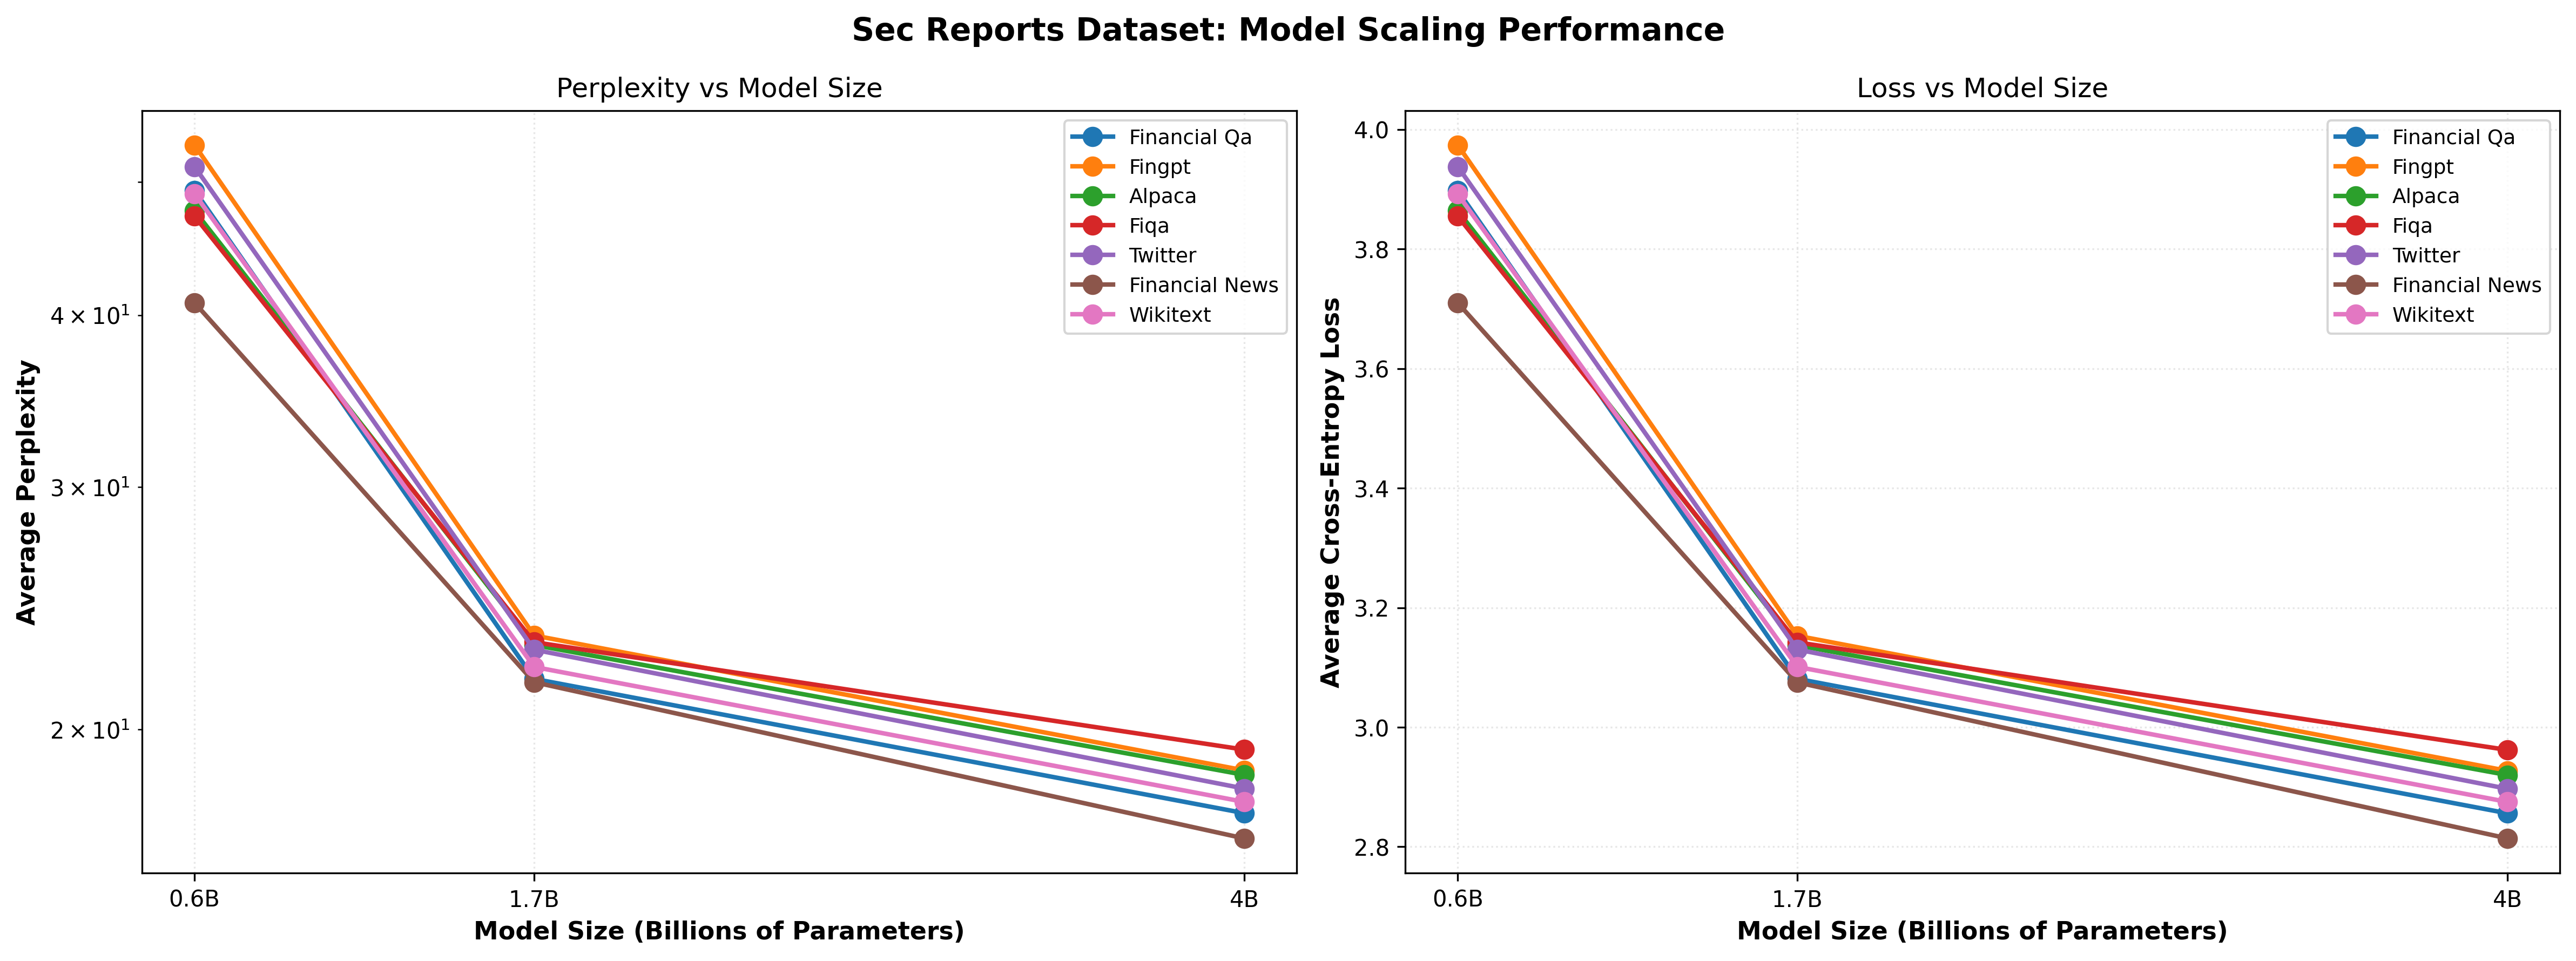
\includegraphics[width=\textwidth]{../thesis/figures/scaling_sec_reports.png}
  \caption{SEC Reports scaling.}\label{fig:scaling_sec_reports}
\end{figure}

{\tighttable
% SEC Reports Dataset: Evaluation Results
% Training: SEC Reports (SEC 10-K/10-Q filings, 80M tokens)
% All models trained with LR=2e-5

\begin{table}[h]
\centering
\caption[SEC Reports: Evaluation Results]{SEC Reports Dataset: Evaluation Across Multiple Datasets}
\label{tab:sec_reports_results}
\begin{tabular}{l|ccc|ccc}
\hline
\textbf{Eval Dataset} & \multicolumn{3}{c|}{\textbf{Cross-Entropy Loss}} & \multicolumn{3}{c}{\textbf{Perplexity}} \\
\cline{2-4} \cline{5-7}
  & \textbf{0.6B} & \textbf{1.7B} & \textbf{4B} & \textbf{0.6B} & \textbf{1.7B} & \textbf{4B} \\
Alpaca & 3.86 & 3.14 & \textbf{2.92} & 47.65 & \textbf{23.04} & \textbf{18.54} \\
Financial News & 3.71 & 3.08 & \textbf{2.81} & 40.85 & \textbf{21.65} & \textbf{16.67} \\
Financial Qa & 3.90 & 3.08 & \textbf{2.86} & 49.30 & \textbf{21.77} & \textbf{17.39} \\
Fingpt & 3.97 & 3.15 & \textbf{2.93} & 53.18 & \textbf{23.41} & \textbf{18.68} \\
Fiqa & 3.85 & 3.14 & \textbf{2.96} & 47.22 & \textbf{23.15} & \textbf{19.34} \\
Twitter & 3.94 & 3.13 & \textbf{2.90} & 51.30 & \textbf{22.86} & \textbf{18.12} \\
Wikitext & 3.89 & 3.10 & \textbf{2.88} & 49.02 & \textbf{22.21} & \textbf{17.72} \\
\hline
\end{tabular}
\end{table}

}

\begin{figure}[H]
  \centering
  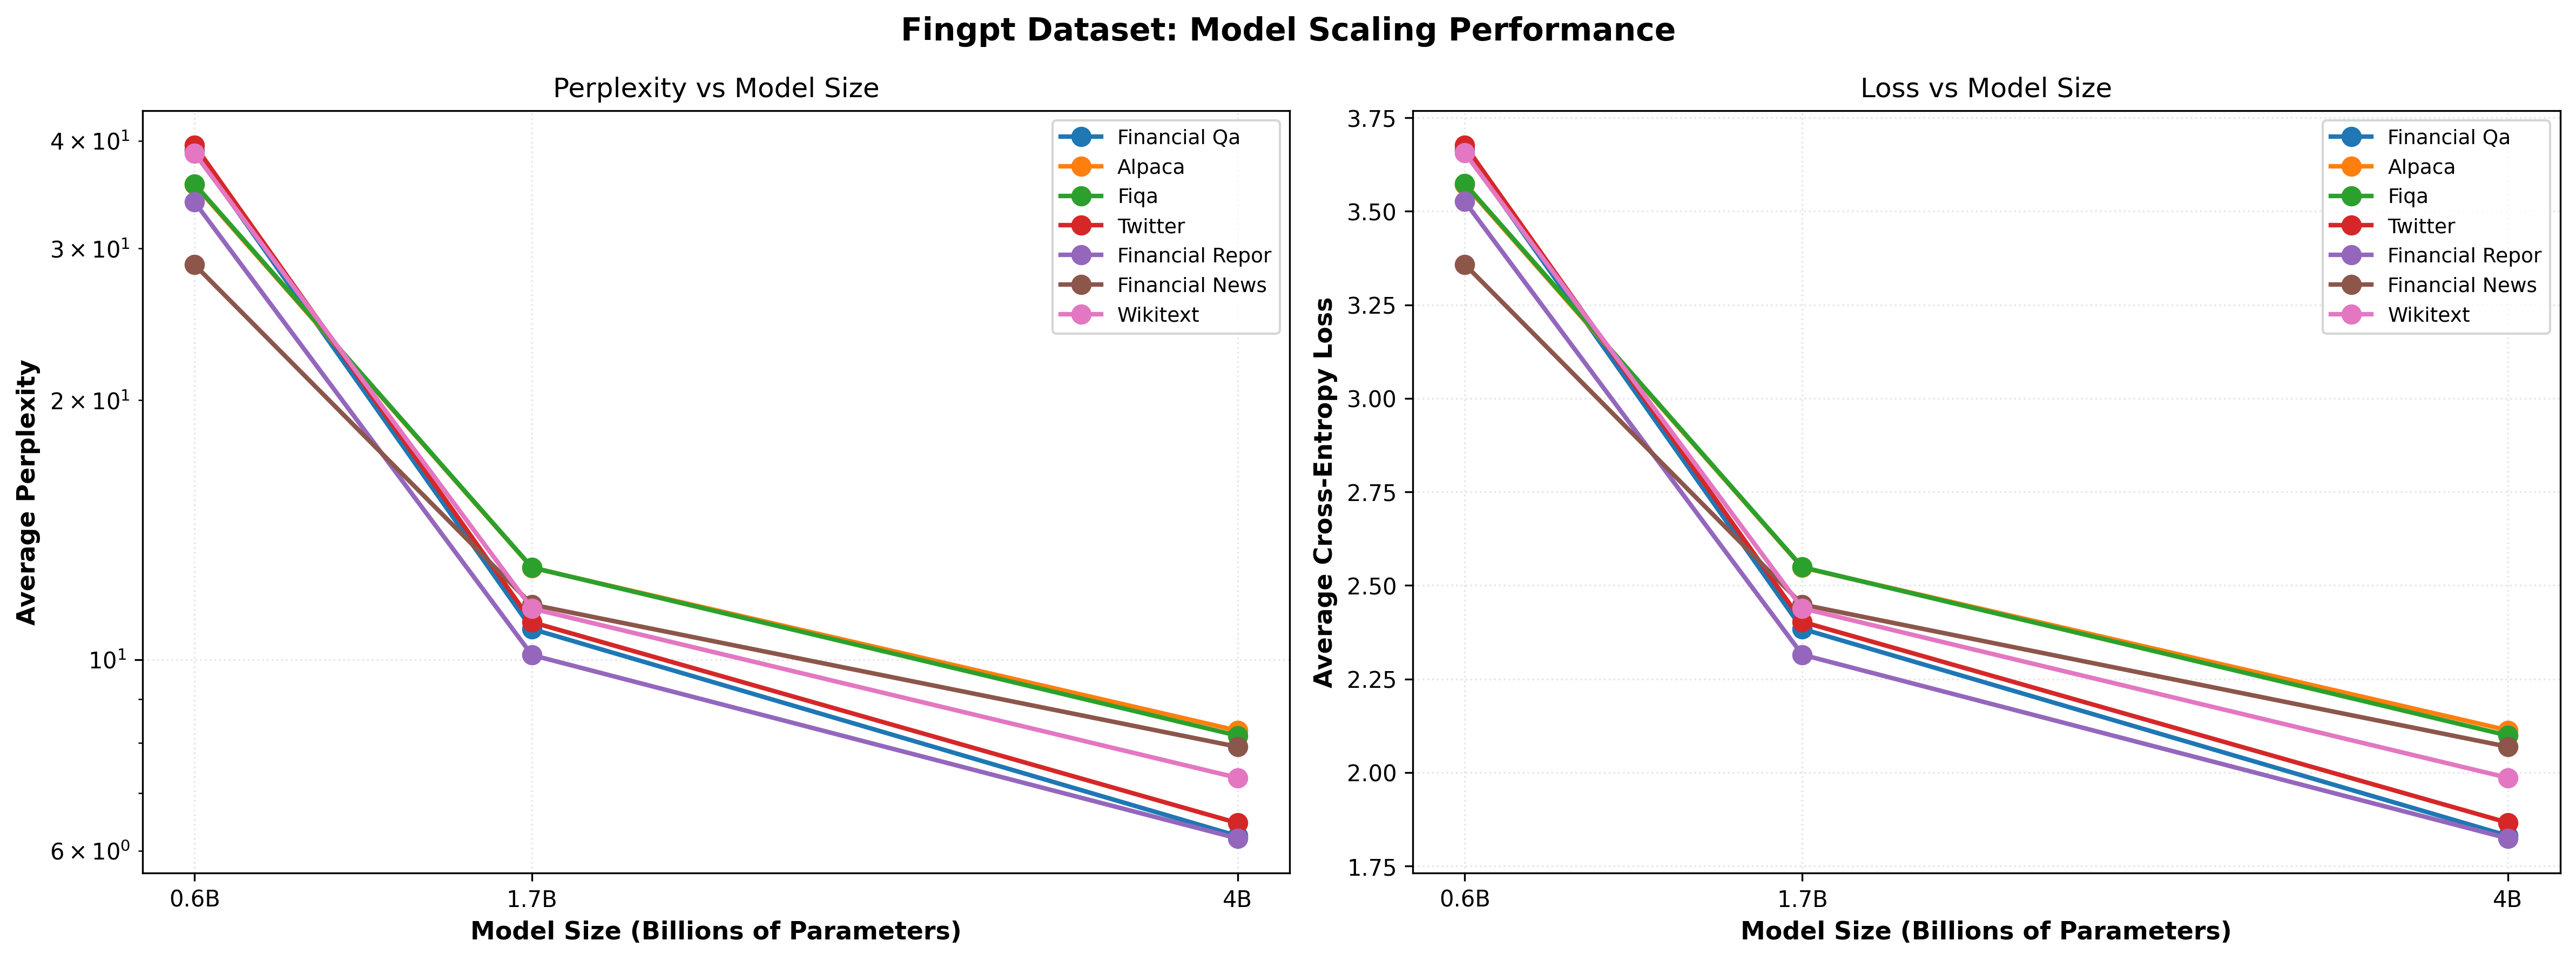
\includegraphics[width=\textwidth]{../thesis/figures/scaling_fingpt.png}
  \caption{FinGPT instruction mixture scaling.}\label{fig:scaling_fingpt}
\end{figure}

{\tighttable
% FinGPT Sentiment Dataset: Evaluation Results
% Training: FinGPT Sentiment (FinGPT/fingpt-sentiment-train, 19M tokens)
% All models trained with LR=2e-5

\begin{table}[h]
\centering
\caption{FinGPT Sentiment Dataset: Evaluation Across Multiple Datasets}
\label{tab:fingpt_results}
\begin{tabular}{l|ccc|ccc}
\hline
\textbf{Eval Dataset} & \multicolumn{3}{c|}{\textbf{Cross-Entropy Loss}} & \multicolumn{3}{c}{\textbf{Perplexity}} \\n\cline{2-4} \cline{5-7}
  & \textbf{0.6B} & \textbf{1.7B} & \textbf{4B} & \textbf{0.6B} & \textbf{1.7B} & \textbf{4B} \\
Alpaca & 3.57 & 2.55 & \textbf{2.11} & 35.55 & \textbf{12.78} & \textbf{8.27} \
 Financial News & 3.36 & 2.45 & \textbf{2.07} & 28.72 & \textbf{11.58} & \textbf{7.92} \
 Financial Qa & 3.66 & 2.38 & \textbf{1.83} & 38.96 & \textbf{10.85} & \textbf{6.24} \
 Financial Repor & 3.53 & 2.31 & \textbf{1.82} & 33.97 & \textbf{10.12} & \textbf{6.20} \
 Fiqa & 3.57 & 2.55 & \textbf{2.10} & 35.64 & \textbf{12.79} & \textbf{8.16} \
 Twitter & 3.68 & 2.40 & \textbf{1.87} & 39.54 & \textbf{11.05} & \textbf{6.46} \
 Wikitext & 3.66 & 2.44 & \textbf{1.99} & 38.70 & \textbf{11.46} & \textbf{7.29} \
\hline
\end{tabular}
\end{table}

}

\begin{figure}[H]
  \centering
  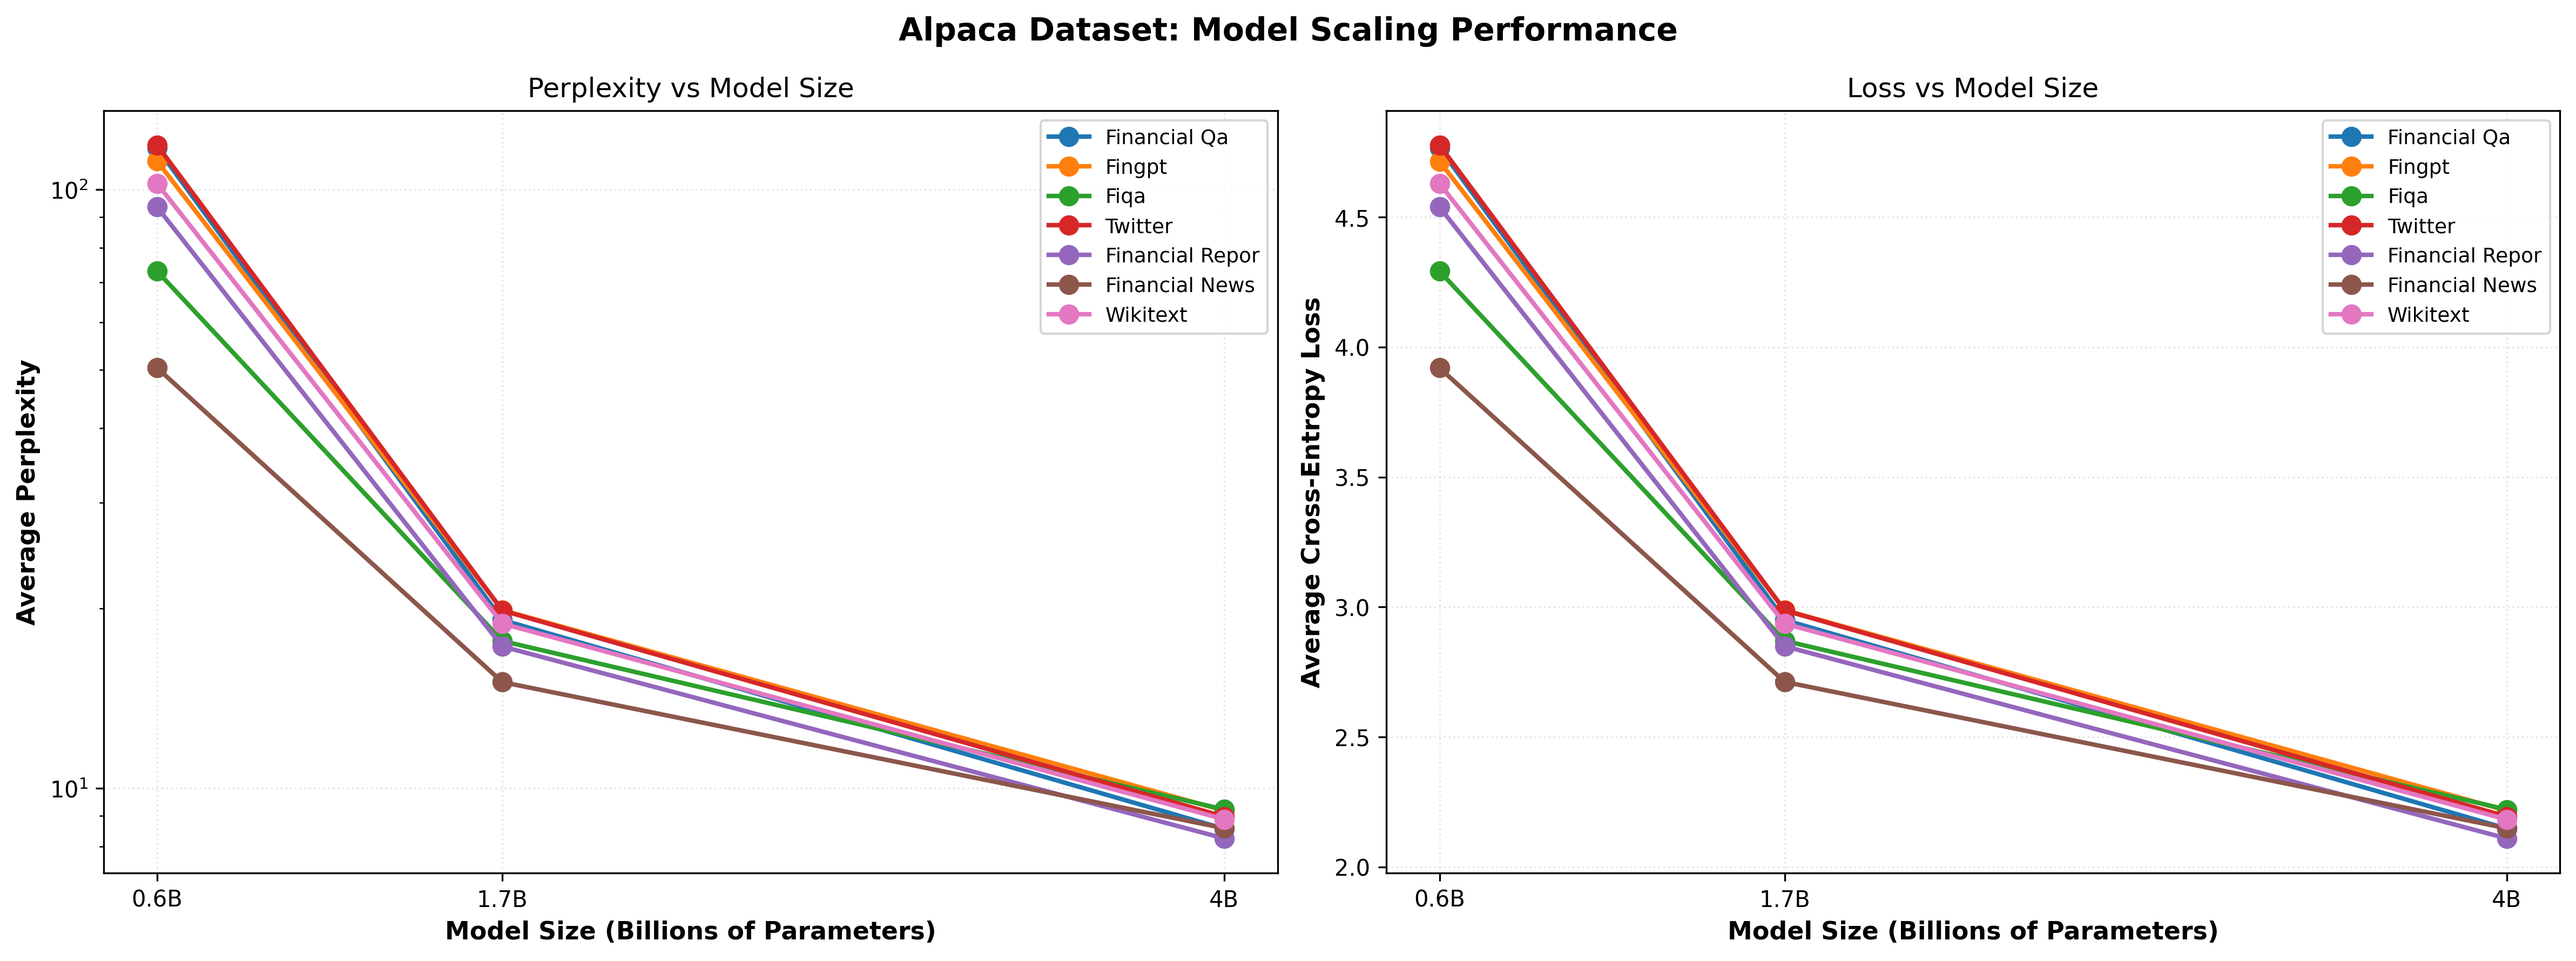
\includegraphics[width=\textwidth]{../thesis/figures/scaling_alpaca.png}
  \caption{Alpaca instruction mixture scaling.}\label{fig:scaling_alpaca}
\end{figure}

{\tighttable
% Finance Alpaca Dataset: Evaluation Results
% Training: Finance Alpaca (gbharti/finance-alpaca, 8.46M tokens)
% All models trained with LR=2e-5

\begin{table}[h]
\centering
\caption[Finance Alpaca: Evaluation Results]{Finance Alpaca Dataset: Evaluation Across Multiple Datasets}
\label{tab:alpaca_results}
\begin{tabular}{l|ccc|ccc}
\hline
\textbf{Eval Dataset} & \multicolumn{3}{c|}{\textbf{Cross-Entropy Loss}} & \multicolumn{3}{c}{\textbf{Perplexity}} \\
\cline{2-4} \cline{5-7}
  & \textbf{0.6B} & \textbf{1.7B} & \textbf{4B} & \textbf{0.6B} & \textbf{1.7B} & \textbf{4B} \\
\textbf{Alpaca} & \textbf{4.15} & \textbf{2.75} & \textbf{2.11} & \textbf{63.73} & \textbf{15.61} & \textbf{8.22} \\
Financial News & 3.92 & 2.71 & 2.15 & 50.40 & 15.05 & 8.58 \\
Financial QA & 4.77 & 2.95 & 2.15 & 117.4 & 19.11 & 8.56 \\
SEC Reports & 4.54 & 2.85 & 2.11 & 93.56 & 17.26 & 8.25 \\
FinGPT & 4.71 & 2.99 & 2.22 & 111.7 & 19.85 & 9.18 \\
FiQA & 4.29 & 2.87 & 2.22 & 73.12 & 17.63 & 9.22 \\
Twitter & 4.78 & 2.99 & 2.19 & 118.7 & 19.82 & 8.97 \\
Wikitext & 4.63 & 2.94 & 2.18 & 102.4 & 18.85 & 8.88 \\
\hline
\textbf{Average} & \textbf{4.47} & \textbf{2.88} & \textbf{2.17} & \textbf{91.37} & \textbf{17.90} & \textbf{8.73} \\
\hline
\end{tabular}
\end{table}
}

\begin{figure}[H]
  \centering
  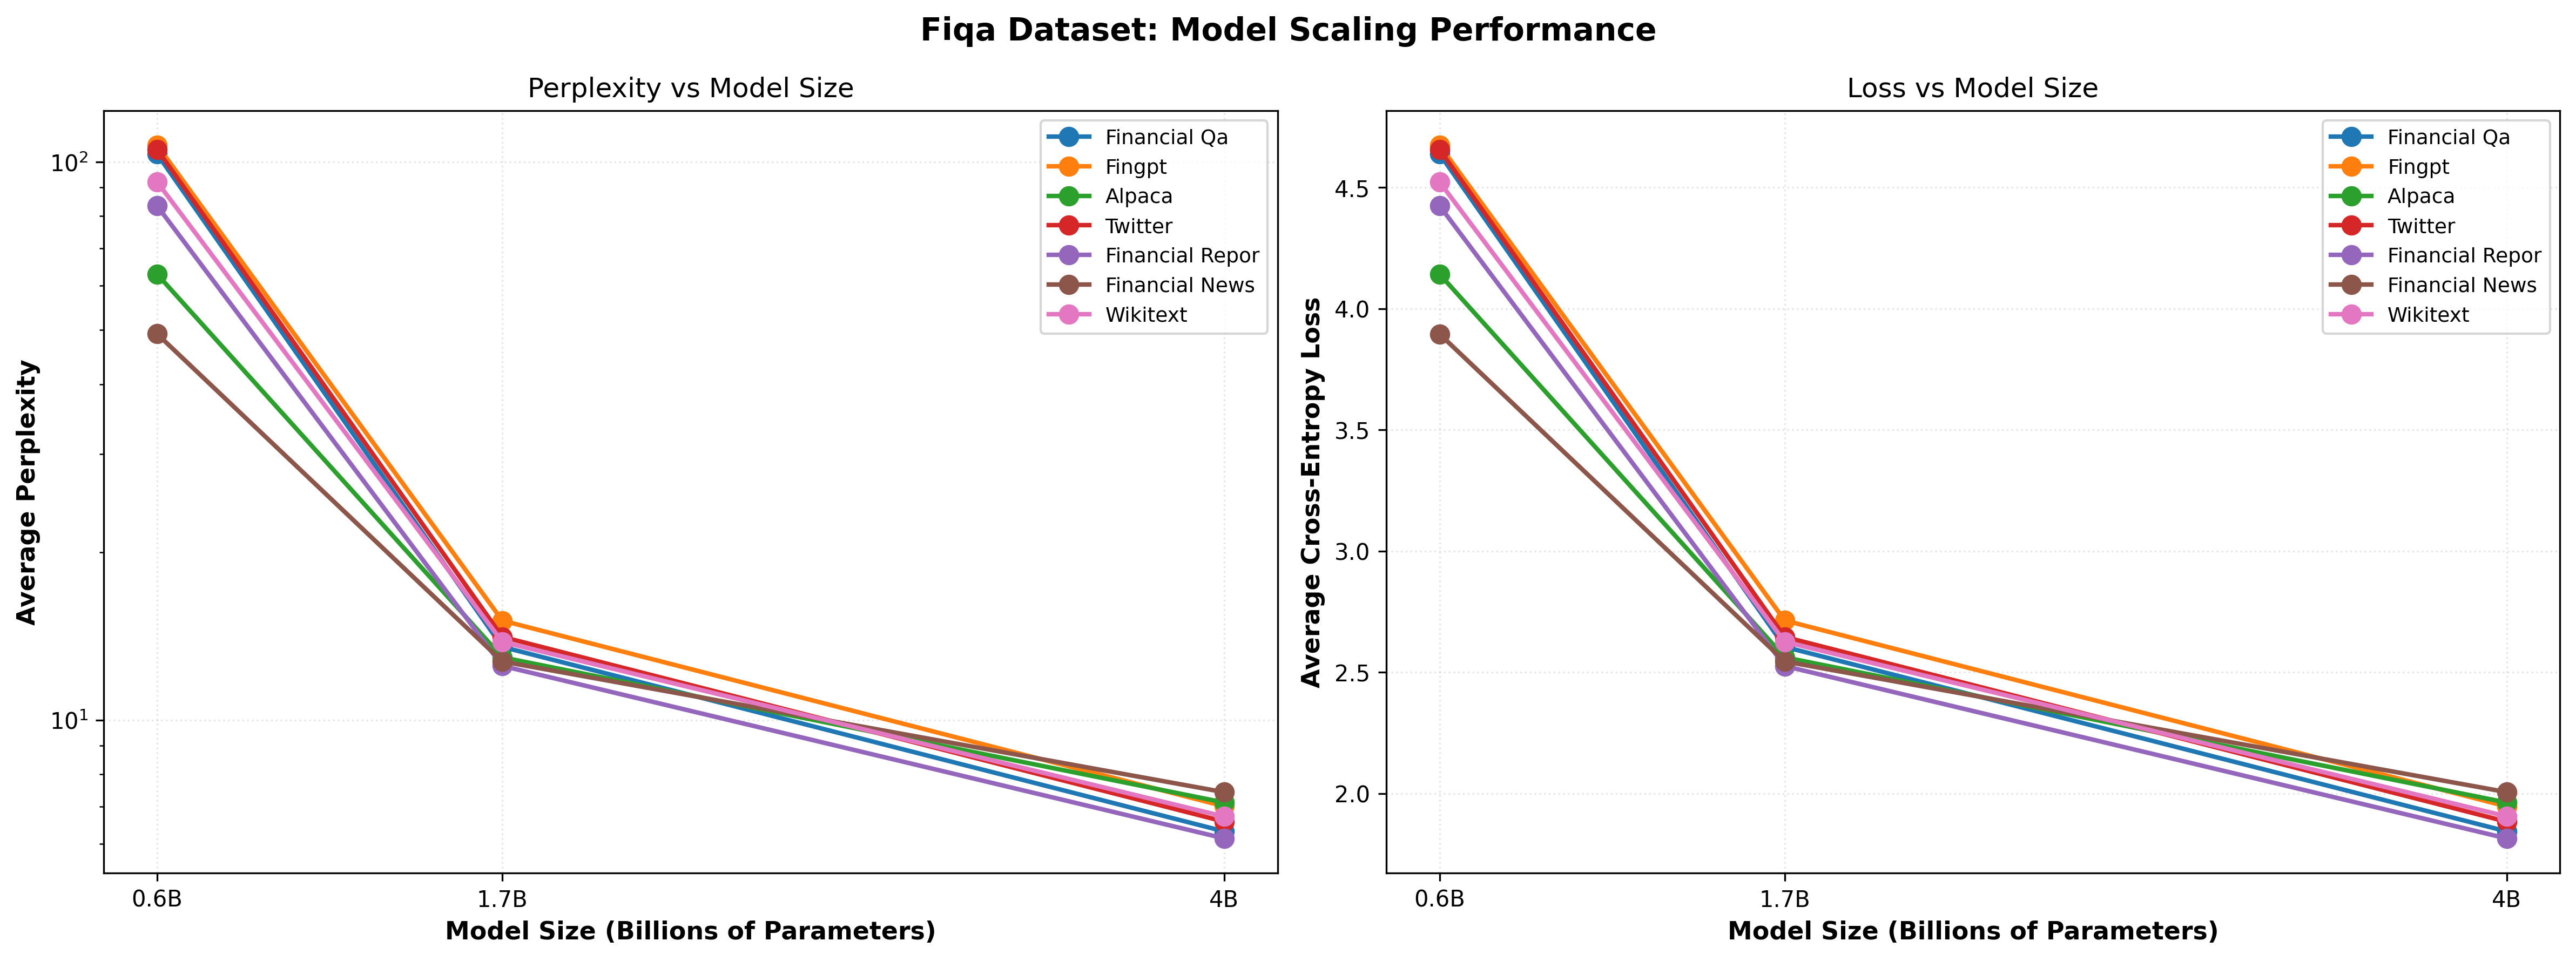
\includegraphics[width=\textwidth]{../thesis/figures/scaling_fiqa.png}
  \caption{FiQA short-form scaling.}\label{fig:scaling_fiqa}
\end{figure}

{\tighttable
% FiQA Dataset: Evaluation Results
% Training: FiQA (FiQA dataset, 4M tokens)
% All models trained with LR=2e-5

\begin{table}[h]
\centering
\caption[FiQA: Evaluation Results]{FiQA Dataset: Evaluation Across Multiple Datasets}
\label{tab:fiqa_results}
\begin{tabular}{l|ccc|ccc}
\hline
\textbf{Eval Dataset} & \multicolumn{3}{c|}{\textbf{Cross-Entropy Loss}} & \multicolumn{3}{c}{\textbf{Perplexity}} \\
\cline{2-4} \cline{5-7}
  & \textbf{0.6B} & \textbf{1.7B} & \textbf{4B} & \textbf{0.6B} & \textbf{1.7B} & \textbf{4B} \\
Alpaca & 4.14 & 2.56 & \textbf{1.96} & 62.97 & \textbf{12.96} & \textbf{7.12} \\
Financial News & 3.90 & 2.54 & \textbf{2.01} & 49.22 & \textbf{12.74} & \textbf{7.43} \\
Financial Qa & 4.64 & 2.60 & \textbf{1.84} & 103.4 & \textbf{13.53} & \textbf{6.32} \\
Financial Repor & 4.42 & 2.53 & \textbf{1.81} & 83.48 & \textbf{12.51} & \textbf{6.14} \\
Fingpt & 4.67 & 2.71 & \textbf{1.95} & 107.2 & \textbf{15.08} & \textbf{7.01} \\
Twitter & 4.66 & 2.65 & \textbf{1.88} & 105.3 & \textbf{14.10} & \textbf{6.58} \\
Wikitext & 4.52 & 2.63 & \textbf{1.91} & 92.13 & \textbf{13.81} & \textbf{6.72} \\
\hline
\end{tabular}
\end{table}

}

{\tighttable
% Financial QA 10K Dataset: Evaluation Results
% Training: Financial QA 10K (virattt/financial-qa-10K, 0.70M tokens)
% All models trained with LR=2e-5

\begin{table}[h]
\centering
\caption[Financial QA 10K: Evaluation Results]{Financial QA 10K Dataset: Evaluation Across Multiple Datasets}
\label{tab:financial_qa_results}
\begin{tabular}{l|ccc|ccc}
\hline
\textbf{Eval Dataset} & \multicolumn{3}{c|}{\textbf{Cross-Entropy Loss}} & \multicolumn{3}{c}{\textbf{Perplexity}} \\
\cline{2-4} \cline{5-7}
  & \textbf{0.6B} & \textbf{1.7B} & \textbf{4B} & \textbf{0.6B} & \textbf{1.7B} & \textbf{4B} \\
\textbf{Financial QA} & \textbf{2.12} & \textbf{2.01} & \textbf{2.12} & \textbf{8.29} & \textbf{7.44} & \textbf{8.29} \\
Alpaca & 2.38 & \textbf{2.23} & 2.29 & 10.82 & \textbf{9.31} & 9.91 \\
Financial News & 2.36 & 2.17 & \textbf{2.13} & 10.60 & \textbf{8.78} & \textbf{8.41} \\
SEC Reports & 2.11 & \textbf{2.00} & 2.11 & 8.21 & \textbf{7.40} & 8.25 \\
FinGPT & 2.31 & \textbf{2.15} & 2.23 & 10.04 & \textbf{8.62} & 9.34 \\
FiQA & 2.40 & \textbf{2.25} & 2.31 & 11.02 & \textbf{9.45} & 10.05 \\
Twitter & 2.21 & \textbf{2.10} & 2.20 & 9.14 & \textbf{8.18} & 8.99 \\
Wikitext & 2.24 & \textbf{2.11} & 2.19 & 9.41 & \textbf{8.23} & 8.89 \\
\hline
\end{tabular}
\end{table}
}
{\tighttable
% Twitter Financial Dataset: Evaluation Results
% Training: Twitter Financial (Financial tweets, 0.3M tokens)
% All models trained with LR=2e-5

\begin{table}[h]
\centering
\caption[Twitter Financial: Evaluation Results]{Twitter Financial Dataset: Evaluation Across Multiple Datasets}
\label{tab:twitter_results}
\begin{tabular}{l|ccc|ccc}
\hline
\textbf{Eval Dataset} & \multicolumn{3}{c|}{\textbf{Cross-Entropy Loss}} & \multicolumn{3}{c}{\textbf{Perplexity}} \\
\cline{2-4} \cline{5-7}
  & \textbf{0.6B} & \textbf{1.7B} & \textbf{4B} & \textbf{0.6B} & \textbf{1.7B} & \textbf{4B} \\
Alpaca & 3.01 & \textbf{2.66} & 2.96 & 20.21 & \textbf{14.33} & 19.20 \\
Financial News & 3.17 & \textbf{2.80} & 2.87 & 23.77 & \textbf{16.48} & 17.67 \\
Financial Qa & 2.46 & \textbf{2.32} & 2.83 & 11.76 & \textbf{10.15} & 16.98 \\
Financial Repor & 2.48 & \textbf{2.32} & 2.80 & 11.95 & \textbf{10.17} & 16.42 \\
Fingpt & 2.74 & \textbf{2.50} & 2.91 & 15.53 & \textbf{12.23} & 18.34 \\
Fiqa & 2.98 & \textbf{2.66} & 3.00 & 19.67 & \textbf{14.26} & 20.09 \\
Wikitext & 2.69 & \textbf{2.47} & 2.88 & 14.74 & \textbf{11.78} & 17.85 \\
\hline
\end{tabular}
\end{table}

}
{\tighttable
% WikiText Dataset: Evaluation Results
% Training: WikiText (WikiText-103, 123.58M tokens)
% All models trained with LR=2e-5

\begin{table}[htbp]
\centering
\caption[WikiText: Evaluation Results]{WikiText Dataset: Evaluation Across Multiple Datasets}
\label{tab:wikitext_results}
\begin{tabular}{l|ccc|ccc}
\hline
\textbf{Eval Dataset} & \multicolumn{3}{c|}{\textbf{Cross-Entropy Loss}} & \multicolumn{3}{c}{\textbf{Perplexity}} \\
\cline{2-4} \cline{5-7}
  & \textbf{0.6B} & \textbf{1.7B} & \textbf{4B} & \textbf{0.6B} & \textbf{1.7B} & \textbf{4B} \\
Alpaca & 2.22 & 3.24 & 3.48 & 9.23 & 25.51 & 32.38 \\
Financial News & 2.62 & 2.93 & 3.37 & 13.70 & 18.78 & 29.19 \\
Financial QA & 3.40 & 10.67 & 3.37 & 29.90 & $\infty$ & 29.08 \\
SEC Reports & 1.39 & 3.27 & 3.44 & 3.99 & 26.46 & 31.23 \\
FinGPT & 1.30 & 2.11 & 3.57 & 3.67 & 8.27 & 35.50 \\
FiQA & 2.07 & 3.14 & 3.53 & 7.89 & 23.15 & 34.03 \\
Twitter & 1.45 & 2.78 & 3.52 & 4.26 & 16.06 & 33.71 \\
\textbf{Wikitext} & \textbf{1.56} & \textbf{3.42} & \textbf{3.30} & \textbf{4.78} & \textbf{30.63} & \textbf{27.19} \\
\hline
\textbf{Average} & \textbf{2.00} & \textbf{3.95} & \textbf{3.45} & \textbf{9.68} & \textbf{$\infty$} & \textbf{31.54} \\
\hline
\end{tabular}
\end{table}
}

Across these tables, 4B wins on the training dataset's own evaluation split (in-domain), but cross-dataset performance depends on format proximity. Short-form datasets (Twitter, Financial QA) show the highest CV and weakest transfer, while long-form (News, SEC) are most robust as standalone pretraining sources.

\section{Cross-Dataset Transfer}
\begin{figure}[H]
  \centering
  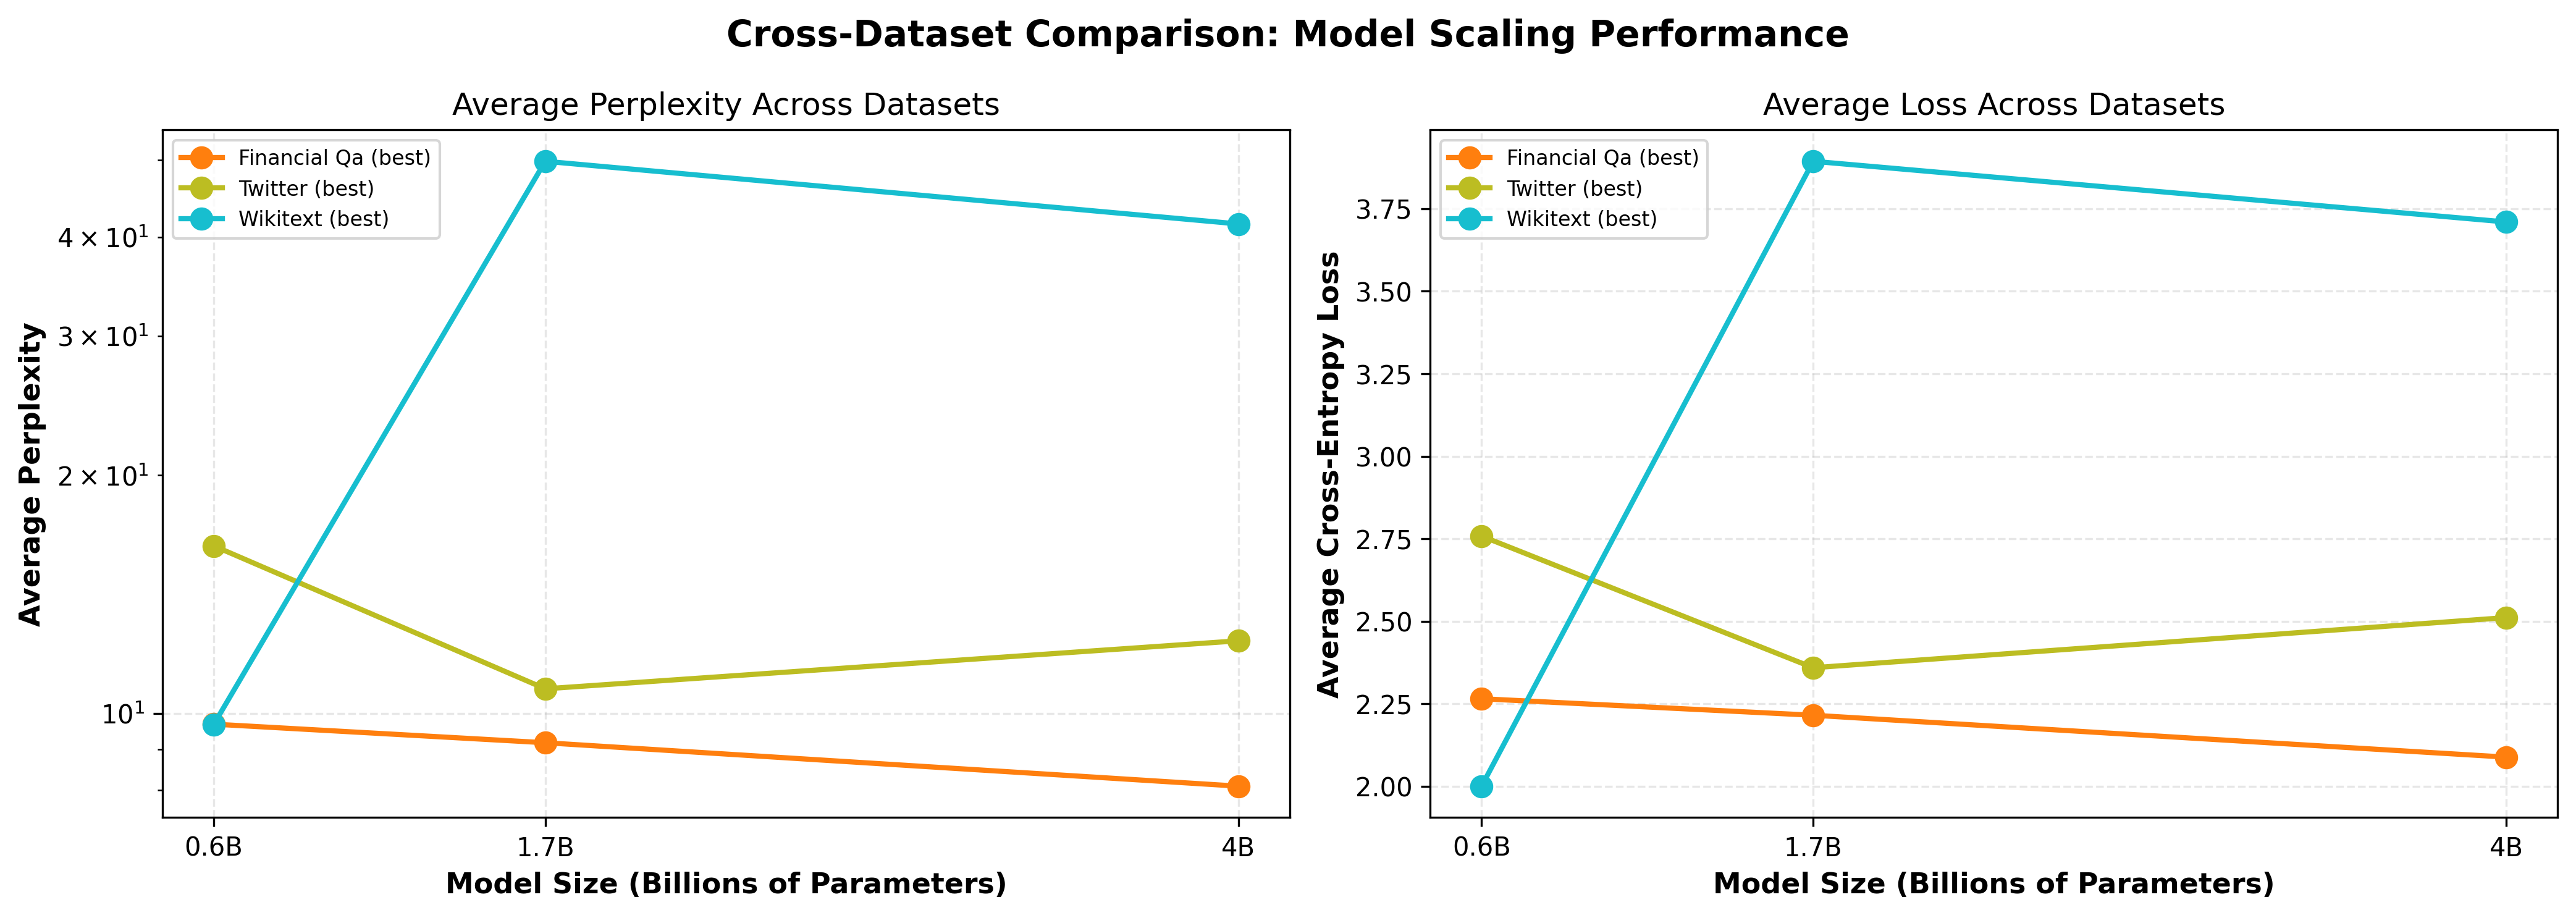
\includegraphics[width=\textwidth]{../thesis/figures/scaling_comparison_all.png}
  \caption{Comparison across training sources.}\label{fig:scaling_comparison_all}
\end{figure}

We analyze transfer by fixing an evaluation dataset and comparing across training sources. Boldface indicates the best training source for each evaluation column.

{\tighttable
% Cross-Dataset Comparison: Financial News as Evaluation Dataset
% Shows which training dataset performs best on Financial News
% Bold values indicate best performance for each model size

\begin{table}[h]
\centering
\caption{Financial News Evaluation: Performance Across Training Datasets}
\label{tab:cross_financial_news}
\begin{tabular}{l|ccc|ccc}
\hline
\textbf{Training Dataset} & \multicolumn{3}{c|}{\textbf{Cross-Entropy Loss}} & \multicolumn{3}{c}{\textbf{Perplexity}} \\n\cline{2-4} \cline{5-7}
  & \textbf{0.6B} & \textbf{1.7B} & \textbf{4B} & \textbf{0.6B} & \textbf{1.7B} & \textbf{4B} \\
Alpaca (2e-5) & 3.92 & 2.71 & 2.15 & 50.40 & 15.05 & 8.58  \
 Financial QA (2e-5) & \textbf{2.36} & \textbf{2.17} & 2.13 & \textbf{10.60} & \textbf{8.78} & 8.41  \
 Financial QA (1.7B: 1e-5, 4B: 5e-6) & \textbf{2.36} & 2.23 & 2.04 & \textbf{10.60} & 9.25 & 7.71  \
 FinGPT (2e-5) & 3.36 & 2.45 & 2.07 & 28.72 & 11.58 & 7.92  \
 FiQA (2e-5) & 3.90 & 2.54 & \textbf{2.01} & 49.22 & 12.74 & \textbf{7.43}  \
 Mixed Financial (2e-5) & 4.03 & 3.05 & 2.63 & 56.35 & 21.19 & 13.84  \
 Mixed Wiki+Financial (2e-5) & 3.65 & 3.13 & 2.77 & 38.68 & 22.79 & 15.91  \
 Financial News (2e-5) & 3.96 & 3.13 & 2.86 & 52.25 & 22.91 & 17.47  \
 SEC Reports (2e-5) & 3.71 & 3.08 & 2.81 & 40.85 & 21.65 & 16.67  \
 Twitter Financial (2e-5) & 3.17 & 2.80 & 2.87 & 23.77 & 16.48 & 17.67  \
 Twitter Financial (1.7B: 1e-5, 4B: 5e-6) & 3.17 & 2.65 & 2.54 & 23.77 & 14.10 & 12.68  \
 WikiText (2e-5) & 2.62 & 2.93 & 3.37 & 13.70 & 18.78 & 29.19  \
 WikiText (1.7B: 5e-6, 4B: 3e-6) & 2.62 & 3.52 & 3.27 & 13.70 & 33.66 & 26.44  \
\hline
\end{tabular}
\end{table}

}

On Financial News evaluation, long-form training sources dominate: News and SEC rows capture most boldface cells. Mixed Financial performs strongly across sizes, reflecting its diversity advantage.

{\tighttable
% Cross-Dataset Comparison: SEC Reports as Evaluation Dataset
% Shows which training dataset performs best on SEC Reports
% Bold values indicate best performance for each model size

\begin{table}[h]
\centering
\caption[SEC Reports Evaluation: Cross-Dataset Performance]{SEC Reports Evaluation: Performance Across Training Datasets}
\label{tab:cross_financial_repor}
\begin{tabular}{l|ccc|ccc}
\hline
\textbf{Training Dataset} & \multicolumn{3}{c|}{\textbf{Cross-Entropy Loss}} & \multicolumn{3}{c}{\textbf{Perplexity}} \\
\cline{2-4} \cline{5-7}
  & \textbf{0.6B} & \textbf{1.7B} & \textbf{4B} & \textbf{0.6B} & \textbf{1.7B} & \textbf{4B} \\
Alpaca (2e-5) & 4.54 & 2.85 & 2.11 & 93.56 & 17.26 & 8.25  \\
Financial QA (2e-5) & 2.11 & \textbf{2.00} & 2.11 & 8.21 & \textbf{7.40} & 8.25  \\
Financial QA (1.7B: 1e-5, 4B: 5e-6) & 2.11 & 2.10 & 2.01 & 8.21 & 8.19 & 7.43  \\
FinGPT (2e-5) & 3.53 & 2.31 & 1.82 & 33.97 & 10.12 & 6.20  \\
FiQA (2e-5) & 4.42 & 2.53 & \textbf{1.81} & 83.48 & 12.51 & \textbf{6.14}  \\
Mixed Financial (2e-5) & 4.94 & 3.58 & 3.11 & 139.62 & 35.83 & 22.36  \\
Mixed Wiki+Financial (2e-5) & 4.35 & 3.69 & 3.33 & 77.57 & 40.17 & 27.91  \\
Financial News (2e-5) & 4.85 & 3.73 & 3.51 & 127.73 & 41.68 & 33.46  \\
SEC Reports (2e-5) & 3.72 & 2.96 & 2.77 & 41.12 & 19.36 & 15.91  \\
Twitter Financial (2e-5) & 2.48 & 2.32 & 2.80 & 11.95 & 10.17 & 16.42  \\
Twitter Financial (1.7B: 1e-5, 4B: 5e-6) & 2.48 & 2.16 & 2.39 & 11.95 & 8.70 & 10.93  \\
WikiText (2e-5) & \textbf{1.39} & 3.27 & 3.44 & \textbf{3.99} & 26.46 & 31.23  \\
WikiText (1.7B: 5e-6, 4B: 3e-6) & \textbf{1.39} & 3.91 & 3.75 & \textbf{3.99} & 49.83 & 42.41  \\
\hline
\end{tabular}
\end{table}

}

On SEC Reports, the pattern mirrors News: long-form training excels. Mixed Financial remains competitive; Mixed Wiki+Financial improves WikiText but rarely wins here.

{\tighttable
% Cross-Dataset Comparison: Alpaca as Evaluation Dataset
% Shows which training dataset performs best on Alpaca
% Bold values indicate best performance for each model size

\begin{table}[htbp]
\centering
\caption[Alpaca Evaluation: Cross-Dataset Performance]{Alpaca Evaluation: Performance Across Training Datasets}
\label{tab:cross_alpaca}
\begin{tabular}{l|ccc|ccc}
\hline
\textbf{Training Dataset} & \multicolumn{3}{c|}{\textbf{Cross-Entropy Loss}} & \multicolumn{3}{c}{\textbf{Perplexity}} \\
\cline{2-4} \cline{5-7}
  & \textbf{0.6B} & \textbf{1.7B} & \textbf{4B} & \textbf{0.6B} & \textbf{1.7B} & \textbf{4B} \\
Alpaca (2e-5) & 4.16 & 2.75 & 2.11 & 63.73 & 15.61 & 8.22  \\
Financial QA (2e-5) & 2.38 & \textbf{2.23} & 2.29 & 10.82 & \textbf{9.31} & 9.91  \\
Financial QA (1.7B: 1e-5, 4B: 5e-6) & 2.38 & 2.29 & 2.18 & 10.82 & 9.92 & 8.88  \\
FinGPT (2e-5) & 3.57 & 2.55 & 2.11 & 35.55 & 12.78 & 8.27  \\
FiQA (2e-5) & 4.14 & 2.56 & \textbf{1.96} & 62.97 & 12.96 & \textbf{7.12}  \\
Mixed Financial (2e-5) & 4.54 & 3.38 & 2.97 & 93.35 & 29.53 & 19.50  \\
Mixed Wiki+Financial (2e-5) & 4.07 & 3.48 & 3.15 & 58.56 & 32.38 & 23.23  \\
Financial News (2e-5) & 4.57 & 3.61 & 3.39 & 96.31 & 36.92 & 29.75  \\
SEC Reports (2e-5) & 3.86 & 3.14 & 2.92 & 47.65 & 23.04 & 18.54  \\
Twitter Financial (2e-5) & 3.01 & 2.66 & 2.96 & 20.21 & 14.33 & 19.20  \\
Twitter Financial (1.7B: 1e-5, 4B: 5e-6) & 3.01 & 2.54 & 2.61 & 20.21 & 12.66 & 13.65  \\
WikiText (2e-5) & \textbf{2.22} & 3.24 & 3.48 & \textbf{9.23} & 25.51 & 32.38  \\
WikiText (1.7B: 5e-6, 4B: 3e-6) & \textbf{2.22} & 3.79 & 3.64 & \textbf{9.23} & 44.22 & 38.06  \\
\hline
\end{tabular}
\end{table}

}
{\tighttable
% Cross-Dataset Comparison: FinGPT as Evaluation Dataset
% Shows which training dataset performs best on FinGPT
% Bold values indicate best performance for each model size

\begin{table}[h]
\centering
\caption[FinGPT Evaluation: Cross-Dataset Performance]{FinGPT Evaluation: Performance Across Training Datasets}
\label{tab:cross_fingpt}
\begin{tabular}{l|ccc|ccc}
\hline
\textbf{Training Dataset} & \multicolumn{3}{c|}{\textbf{Cross-Entropy Loss}} & \multicolumn{3}{c}{\textbf{Perplexity}} \\
\cline{2-4} \cline{5-7}
  & \textbf{0.6B} & \textbf{1.7B} & \textbf{4B} & \textbf{0.6B} & \textbf{1.7B} & \textbf{4B} \\
Alpaca (2e-5) & 4.71 & 2.99 & 2.22 & 111.65 & 19.85 & 9.18  \\
Financial QA (2e-5) & 2.31 & 2.15 & 2.23 & 10.04 & 8.62 & 9.34  \\
Financial QA (1.7B: 1e-5, 4B: 5e-6) & 2.31 & 2.25 & 2.11 & 10.04 & 9.51 & 8.24  \\
FinGPT (2e-5) & 3.49 & 2.26 & \textbf{1.74} & 32.78 & 9.56 & \textbf{5.67}  \\
FiQA (2e-5) & 4.67 & 2.71 & 1.95 & 107.25 & 15.08 & 7.01  \\
Mixed Financial (2e-5) & 5.04 & 3.63 & 3.14 & 153.94 & 37.82 & 23.08  \\
Mixed Wiki+Financial (2e-5) & 4.44 & 3.75 & 3.37 & 84.43 & 42.50 & 28.92  \\
Financial News (2e-5) & 5.08 & 3.90 & 3.64 & 160.92 & 49.56 & 38.03  \\
SEC Reports (2e-5) & 3.97 & 3.15 & 2.93 & 53.18 & 23.41 & 18.68  \\
Twitter Financial (2e-5) & 2.74 & 2.50 & 2.91 & 15.53 & 12.23 & 18.34  \\
Twitter Financial (1.7B: 1e-5, 4B: 5e-6) & 2.74 & 2.34 & 2.54 & 15.53 & 10.41 & 12.69  \\
WikiText (2e-5) & \textbf{1.30} & \textbf{2.11} & 3.57 & \textbf{3.67} & \textbf{8.27} & 35.50  \\
WikiText (1.7B: 5e-6, 4B: 3e-6) & \textbf{1.30} & 4.07 & 3.88 & \textbf{3.67} & 58.55 & 48.30  \\
\hline
\end{tabular}
\end{table}

}

Instruction-formatted evaluations (Alpaca, FinGPT) are best served by instruction-heavy training or diverse mixtures. Mixed Financial at 4B frequently captures boldface, suggesting diversity compensates for format mismatch.

{\tighttable
% Cross-Dataset Comparison: FiQA as Evaluation Dataset
% Shows which training dataset performs best on FiQA
% Bold values indicate best performance for each model size

\begin{table}[h]
\centering
\caption[FiQA Evaluation: Cross-Dataset Performance]{FiQA Evaluation: Performance Across Training Datasets}
\label{tab:cross_fiqa}
\begin{tabular}{l|ccc|ccc}
\hline
\textbf{Training Dataset} & \multicolumn{3}{c|}{\textbf{Cross-Entropy Loss}} & \multicolumn{3}{c}{\textbf{Perplexity}} \\
\cline{2-4} \cline{5-7}
  & \textbf{0.6B} & \textbf{1.7B} & \textbf{4B} & \textbf{0.6B} & \textbf{1.7B} & \textbf{4B} \\
Alpaca (2e-5) & 4.29 & 2.87 & 2.22 & 73.12 & 17.63 & 9.22  \\
Financial QA (2e-5) & 2.40 & \textbf{2.25} & 2.31 & 11.02 & \textbf{9.45} & 10.05  \\
Financial QA (1.7B: 1e-5, 4B: 5e-6) & 2.40 & 2.31 & 2.19 & 11.02 & 10.10 & 8.93  \\
FinGPT (2e-5) & 3.57 & 2.55 & 2.10 & 35.64 & 12.79 & 8.16  \\
FiQA (2e-5) & 4.17 & 2.56 & \textbf{1.96} & 64.75 & 12.99 & \textbf{7.08}  \\
Mixed Financial (2e-5) & 4.63 & 3.46 & 3.05 & 102.47 & 31.85 & 21.20  \\
Mixed Wiki+Financial (2e-5) & 4.14 & 3.56 & 3.24 & 63.03 & 35.04 & 25.61  \\
Financial News (2e-5) & 4.62 & 3.65 & 3.46 & 101.32 & 38.68 & 31.69  \\
SEC Reports (2e-5) & 3.85 & 3.14 & 2.96 & 47.22 & 23.15 & 19.34  \\
Twitter Financial (2e-5) & 2.98 & 2.66 & 3.00 & 19.67 & 14.26 & 20.09  \\
Twitter Financial (1.7B: 1e-5, 4B: 5e-6) & 2.98 & 2.50 & 2.61 & 19.67 & 12.20 & 13.61  \\
WikiText (2e-5) & \textbf{2.07} & 3.14 & 3.53 & \textbf{7.89} & 23.15 & 34.03  \\
WikiText (1.7B: 5e-6, 4B: 3e-6) & \textbf{2.07} & 3.85 & 3.74 & \textbf{7.89} & 46.81 & 42.04  \\
\hline
\end{tabular}
\end{table}

}
{\tighttable
% Cross-Dataset Comparison: Financial QA as Evaluation Dataset
% Shows which training dataset performs best on Financial QA
% Bold values indicate best performance for each model size

\begin{table}[h]
\centering
\caption{Financial QA Evaluation: Performance Across Training Datasets}
\label{tab:cross_financial_qa}
\resizebox{\textwidth}{!}{
\begin{tabular}{l|ccc|ccc}
\toprule
\multirow{2}{*}{\textbf{Training Dataset}} &
\multicolumn{3}{c|}{\textbf{Cross-Entropy Loss}} &
\multicolumn{3}{c}{\textbf{Perplexity}} \\
\cmidrule(lr){2-4} \cmidrule(lr){5-7}
& \textbf{0.6B} & \textbf{1.7B} & \textbf{4B} & \textbf{0.6B} & \textbf{1.7B} & \textbf{4B} \\
\midrule
Alpaca (2e-5) & 4.77 & 2.95 & 2.15 & 117.40 & 19.11 & 8.56 \\
Financial QA (2e-5) & \textbf{2.12} & \textbf{2.01} & 2.12 & \textbf{8.29} & \textbf{7.44} & 8.29 \\
Financial QA (1.7B: 1e-5, 4B: 5e-6) & \textbf{2.12} & 2.12 & 2.01 & \textbf{8.29} & 8.29 & 7.43 \\
FinGPT (2e-5) & 3.66 & 2.38 & \textbf{1.83} & 38.96 & 10.85 & \textbf{6.24} \\
FiQA (2e-5) & 4.64 & 2.60 & 1.84 & 103.40 & 13.53 & 6.32 \\
Mixed Financial (2e-5) & 5.21 & 3.75 & 3.23 & 183.72 & 42.30 & 25.14 \\
Mixed Wiki+Financial (2e-5) & 4.58 & 3.87 & 3.46 & 97.49 & 47.94 & 31.76 \\
Financial News (2e-5) & 5.11 & 3.90 & 3.66 & 166.10 & 49.53 & 38.90 \\
SEC Reports (2e-5) & 3.90 & 3.08 & 2.86 & 49.30 & 21.77 & 17.39 \\
Twitter Financial (2e-5) & 2.46 & 2.32 & 2.83 & 11.76 & 10.15 & 16.98 \\
Twitter Financial (1.7B: 1e-5, 4B: 5e-6) & 2.46 & 2.16 & 2.43 & 11.76 & 8.69 & 11.39 \\
WikiText (2e-5) & 3.40 & 10.67 & 3.37 & 29.90 & $\infty$ & 29.08 \\
WikiText (1.7B: 5e-6, 4B: 3e-6) & 3.40 & 4.07 & 3.87 & 29.90 & 58.33 & 47.98 \\
\bottomrule
\end{tabular}
}
\end{table}

}

Short Q\&A evaluations (FiQA, Financial QA) show mixed results: specialized training wins in-distribution, but diverse mixtures perform robustly. Small single-dataset training is brittle (high CV) and underperforms off-format.

{\tighttable
% Cross-Dataset Comparison: Twitter Financial as Evaluation Dataset
% Shows which training dataset performs best on Twitter Financial
% Bold values indicate best performance for each model size

\begin{table}[h]
\centering
\caption{Twitter Financial Evaluation: Performance Across Training Datasets}
\label{tab:cross_twitter}
\resizebox{\textwidth}{!}{
\begin{tabular}{l|ccc|ccc}
\toprule
\multirow{2}{*}{\textbf{Training Dataset}} &
\multicolumn{3}{c|}{\textbf{Cross-Entropy Loss}} &
\multicolumn{3}{c}{\textbf{Perplexity}} \\
\cmidrule(lr){2-4} \cmidrule(lr){5-7}
& \textbf{0.6B} & \textbf{1.7B} & \textbf{4B} & \textbf{0.6B} & \textbf{1.7B} & \textbf{4B} \\
\midrule
Alpaca (2e-5) & 4.78 & 2.99 & 2.19 & 118.74 & 19.82 & 8.97 \\
Financial QA (2e-5) & 2.21 & \textbf{2.10} & 2.20 & 9.14 & \textbf{8.18} & 8.99 \\
Financial QA (1.7B: 1e-5, 4B: 5e-6) & 2.21 & 2.21 & 2.09 & 9.14 & 9.10 & 8.05 \\
FinGPT (2e-5) & 3.68 & 2.40 & \textbf{1.87} & 39.54 & 11.05 & \textbf{6.46} \\
FiQA (2e-5) & 4.66 & 2.65 & 1.88 & 105.32 & 14.10 & 6.58 \\
Mixed Financial (2e-5) & 5.21 & 3.76 & 3.25 & 182.63 & 42.91 & 25.72 \\
Mixed Wiki+Financial (2e-5) & 4.59 & 3.88 & 3.48 & 98.13 & 48.42 & 32.48 \\
Financial News (2e-5) & 5.11 & 3.91 & 3.66 & 165.22 & 49.88 & 38.98 \\
SEC Reports (2e-5) & 3.94 & 3.13 & 2.90 & 51.30 & 22.86 & 18.12 \\
Twitter Financial (2e-5) & 2.53 & 2.40 & 2.88 & 12.60 & 11.02 & 17.83 \\
Twitter Financial (1.7B: 1e-5, 4B: 5e-6) & 2.53 & 2.22 & 2.47 & 12.60 & 9.21 & 11.81 \\
WikiText (2e-5) & \textbf{1.45} & 2.78 & 3.52 & \textbf{4.26} & 16.06 & 33.71 \\
WikiText (1.7B: 5e-6, 4B: 3e-6) & \textbf{1.45} & 4.08 & 3.88 & \textbf{4.26} & 58.98 & 48.48 \\
\bottomrule
\end{tabular}
}
\end{table}

}

Twitter is an outlier: the Twitter-trained row wins on its own column but transfers poorly elsewhere, and other training sources perform weakly on Twitter. This underscores format isolation in micro-text.

{\tighttable
% Cross-Dataset Comparison: WikiText as Evaluation Dataset
% Shows which training dataset performs best on WikiText
% Bold values indicate best performance for each model size

\begin{table}[h]
\centering
\caption{WikiText Evaluation: Performance Across Training Datasets}
\label{tab:cross_wikitext}
\begin{tabular}{l|ccc|ccc}
\hline
\textbf{Training Dataset} & \multicolumn{3}{c|}{\textbf{Cross-Entropy Loss}} & \multicolumn{3}{c}{\textbf{Perplexity}} \\n\cline{2-4} \cline{5-7}
  & \textbf{0.6B} & \textbf{1.7B} & \textbf{4B} & \textbf{0.6B} & \textbf{1.7B} & \textbf{4B} \\
Alpaca (2e-5) & 4.63 & 2.94 & 2.18 & 102.41 & 18.85 & 8.88  \
 Financial QA (2e-5) & 2.24 & \textbf{2.11} & 2.19 & 9.41 & \textbf{8.23} & 8.89  \
 Financial QA (1.7B: 1e-5, 4B: 5e-6) & 2.24 & 2.21 & 2.08 & 9.41 & 9.08 & 8.00  \
 FinGPT (2e-5) & 3.66 & 2.44 & 1.99 & 38.70 & 11.46 & 7.29  \
 FiQA (2e-5) & 4.52 & 2.63 & \textbf{1.91} & 92.13 & 13.81 & \textbf{6.72}  \
 Mixed Wiki+Financial (2e-5) & 4.41 & 3.74 & 3.32 & 82.10 & 41.95 & 27.72  \
 Financial News (2e-5) & 4.95 & 3.81 & 3.54 & 140.71 & 45.17 & 34.33  \
 SEC Reports (2e-5) & 3.89 & 3.10 & 2.88 & 49.02 & 22.21 & 17.72  \
 Twitter Financial (2e-5) & 2.69 & 2.47 & 2.88 & 14.74 & 11.78 & 17.85  \
 Twitter Financial (1.7B: 1e-5, 4B: 5e-6) & 2.69 & 2.30 & 2.49 & 14.74 & 9.94 & 12.02  \
 WikiText (2e-5) & \textbf{1.56} & 3.42 & 3.30 & \textbf{4.78} & 30.63 & 27.19  \
 WikiText (1.7B: 5e-6, 4B: 3e-6) & \textbf{1.56} & 3.88 & 3.65 & \textbf{4.78} & 48.44 & 38.60  \
\hline
\end{tabular}
\end{table}

}

On WikiText, general-domain or Mixed Wiki+Financial training rows win, as expected. Mixed Financial trades a slight general-domain loss for significant financial gains, which is favorable for finance-centric applications.
